\chapter{IMPLEMENTATION AND TESTING}
\label{ch:implementation-testing}

\ChapterSection{Implementation}

The system architecture, data models, API design, mobile application structure, and integrated
diagnosis workflow are described in Chapter~4. This chapter reports implementation outcomes,
testing evidence, and quantitative results for each subsystem rather than re-describing the
design itself.

\ChapterSubsection{Tools Used}

The implementation uses separate toolchains for model development, backend services, mobile
delivery, data storage, and report preparation. Table~\ref{tab:implementation-tools-used}
summarizes the tools used in the completed project.

{\small
\renewcommand{\arraystretch}{1.3}
\begin{xltabular}{\textwidth}{@{} l L @{}}
\caption{Tools used for implementation}\label{tab:implementation-tools-used}\\
\toprule
\textbf{Category} & \textbf{Tools and platforms} \\
\midrule
\endfirsthead
\multicolumn{2}{l}{\footnotesize\textit{Table \thetable{} \textemdash{} continued from previous page}}\\[3pt]
\toprule
\textbf{Category} & \textbf{Tools and platforms} \\
\midrule
\endhead
\endfoot
\bottomrule
\endlastfoot
Model development & Python, PyTorch, Ultralytics YOLOv8, Hugging Face Transformers, PEFT/LoRA, TRL, vLLM, TensorFlow Lite export tooling \\
Backend development & TypeScript, Node.js, Express, Mongoose, Zod, Multer, JWT, Cloudinary, Google AI client integration \\
Mobile development & React Native, Expo, Expo Router, TanStack Query, i18next, VisionCamera, react-native-fast-tflite, SQLite \\
Databases and storage & MongoDB through Mongoose models, mobile SQLite, Cloudinary image storage, local model and dataset artifacts \\
Testing and validation & Pytest, Jest, Supertest, MongoDB Memory Server, VLM inference API tests, physical Android-device testing \\
Documentation and design artifacts & LaTeX, BibLaTeX, generated architecture diagrams, source-level contract review, Git-based revision tracking \\
\end{xltabular}
}

\ChapterSubsection{Implementation Details of Modules}

The implementation is organized into four primary modules. The YOLO module prepares the
plant-part detection dataset, trains the detector, evaluates threshold behavior, and exports
TFLite variants. The VLM module builds Qwen-format image-text records, fine-tunes
Qwen2.5-VL-3B with LoRA adapters, exposes inference through a FastAPI gateway, and validates
canonical-label parseability. The backend module implements route groups, validation,
authentication, persistence, VLM inference calls, advisory generation, and structured diagnosis
response assembly. The mobile module implements onboarding, scan capture, preview and editing,
network-aware diagnosis, SQLite-backed offline queues, crop records, result presentation,
reminders, sharing, PDF export, and on-device TFLite model loading.

\ChapterSection{Testing}

\ChapterSubsection{Test Cases for Unit Testing}

Unit-level testing focuses on components whose behavior can be checked without running the
complete distributed system. Table~\ref{tab:unit-testing-cases} lists the main implemented
unit-test targets and the behavior each target verifies.

{\small
\renewcommand{\arraystretch}{1.3}
\begin{xltabular}{\textwidth}{@{} l L L @{}}
\caption{Unit testing cases}\label{tab:unit-testing-cases}\\
\toprule
\textbf{Area} & \textbf{Test focus} & \textbf{Expected behavior} \\
\midrule
\endfirsthead
\multicolumn{3}{l}{\footnotesize\textit{Table \thetable{} \textemdash{} continued from previous page}}\\[3pt]
\toprule
\textbf{Area} & \textbf{Test focus} & \textbf{Expected behavior} \\
\midrule
\endhead
\endfoot
\bottomrule
\endlastfoot
YOLO utilities & Data-YAML loading, dataset input resolution, IoU computation, prediction--ground-truth matching & Dataset metadata and validation helpers return consistent class mappings, matches, misses, and false predictions \\
YOLO pipeline & Quantization manifests, model-packaging paths, validation wiring & Exported artifacts and validation inputs are resolved without breaking pipeline contracts \\
VLM utilities & Qwen record loading, split resolution, JSON extraction, canonical-label parsing & Training and validation records resolve image paths and mark unparseable predictions as \texttt{\_\_parse\_error\_\_} \\
VLM runtime & Training dataset resolver, LoRA target selection, runtime compatibility checks & Fine-tuning configuration resolves usable dataset paths and adapter targets without selecting visual modules \\
Backend services & Scan-service behavior and diagnosis parsing helpers & Service logic preserves ownership rules, validates inputs, normalizes model output, and returns expected response fields \\
Mobile inference utilities & TFLite/ONNX inference helpers and detection validation utilities & Model-loading, confidence filtering, and detection-result validation follow configured thresholds \\
\end{xltabular}
}

\ChapterSubsection{Test Cases for System Testing}

Krishi Vaidya is validated through five categories of evidence: model-performance metrics,
dataset and pipeline integrity checks, automated backend and API tests, mobile source and
device-level checks, and integration-boundary verification. Each category addresses a different
reliability claim, and no single metric covers the full system.

\subsubsection{YOLO Validation}

The YOLO subsystem carries the strongest quantitative evidence in the project. Validation
artifacts include training dynamics, best-epoch metrics, threshold analysis, quantized model
comparisons, per-class breakdowns, latency measurements, confusion matrices, and error-category
analysis. Figure~\ref{fig:yolo-validation-evaluation-flow} shows the validation pipeline.



Automated pytest tests verify data-YAML loading, image collection, IoU computation,
prediction--ground-truth matching, quantization manifests, and model-packaging behavior.
These tests support the reliability of the validation tooling itself, while the quantitative
outputs support detector-performance claims.

\subsubsection{VLM Validation}

The VLM was validated at two levels. Dataset validation confirmed 13,294 images, 6,647 Qwen
records, zero decode failures, and zero missing images---establishing structural usability of
the exported training data. Figure~\ref{fig:vlm-validation-evaluation-flow} shows the
validation flow.
\begin{figure}[H]
\centering

\includegraphics[height=0.4\textheight,keepaspectratio,width=\textwidth]{data/flow_digram_data/build/yolo/04_validation_evaluation_flow.pdf}
\caption{YOLO validation and evaluation flow showing metric computation, threshold analysis, and validation outputs.}
\label{fig:yolo-validation-evaluation-flow}
\end{figure}
\begin{figure}[H]
\centering

\includegraphics[height=0.4\textheight,keepaspectratio,width=\textwidth]{data/flow_digram_data/build/vlm/05_validation_evaluation_flow.pdf}
\caption{VLM validation and evaluation flow showing dataset checks, prediction validation, and parse-error handling.}
\label{fig:vlm-validation-evaluation-flow}
\end{figure}

Prediction validation on the 798-example test split yielded accuracy of 0.1303, macro F1 of
0.2465, and 540 parse errors. These results define the current reliability boundary: the
training pipeline works, but a three-epoch LoRA run on curated online data does not yet produce
a diagnostically mature classifier. The VLM repository contains 46 Python test functions,
including 11 dedicated to inference API route behavior covering health, readiness, authentication,
scope validation, image rejection, response mapping, and rate limiting.

\subsubsection{Backend and Integration Validation}

Backend automated tests focus on the scan domain. Twenty-one scan-service unit tests and 26
scan-route integration tests run against MongoDB Memory Server, covering creation, ownership,
filtering, pagination, resolution, follow-up linkage, and grouping. Test coverage was
concentrated on the core scan lifecycle; remaining domains rely on manual verification.

Integration validation combined source inspection, contract review, and distributed runtime
execution. The VLM gateway was deployed on Lightning.ai, the database on Supabase, and the
backend served locally via ngrok. This setup verified the complete mobile-to-cloud request
lifecycle, including offline-to-online queue recovery.

\subsubsection{Mobile Validation}

Source inspection verifies the route hierarchy, provider setup, SQLite schema, offline queue,
sync manager, and model-asset loading paths. Physical-device testing confirms the scan,
diagnosis, settings, crop, and offline recovery workflows. An ONNX YOLO engine test harness
provides inference validation utilities for model loading, warmup, and detection checks.

\ChapterSection{Result Analysis}

\ChapterSubsection{YOLO Training Results}

\subsubsection{Training Dynamics}

The YOLO detector trained for 100 epochs over 7.12 hours. The best recorded epoch was epoch
100, indicating that the run completed its full schedule without early termination.
Figure~\ref{fig:yolo-training-dynamics} shows loss reduction and detection-metric progression
across training. The model improved substantially from early epochs and stabilized toward the
end, with the best mAP@50-95 recorded at the final epoch.

\begin{figure}[H]
\centering
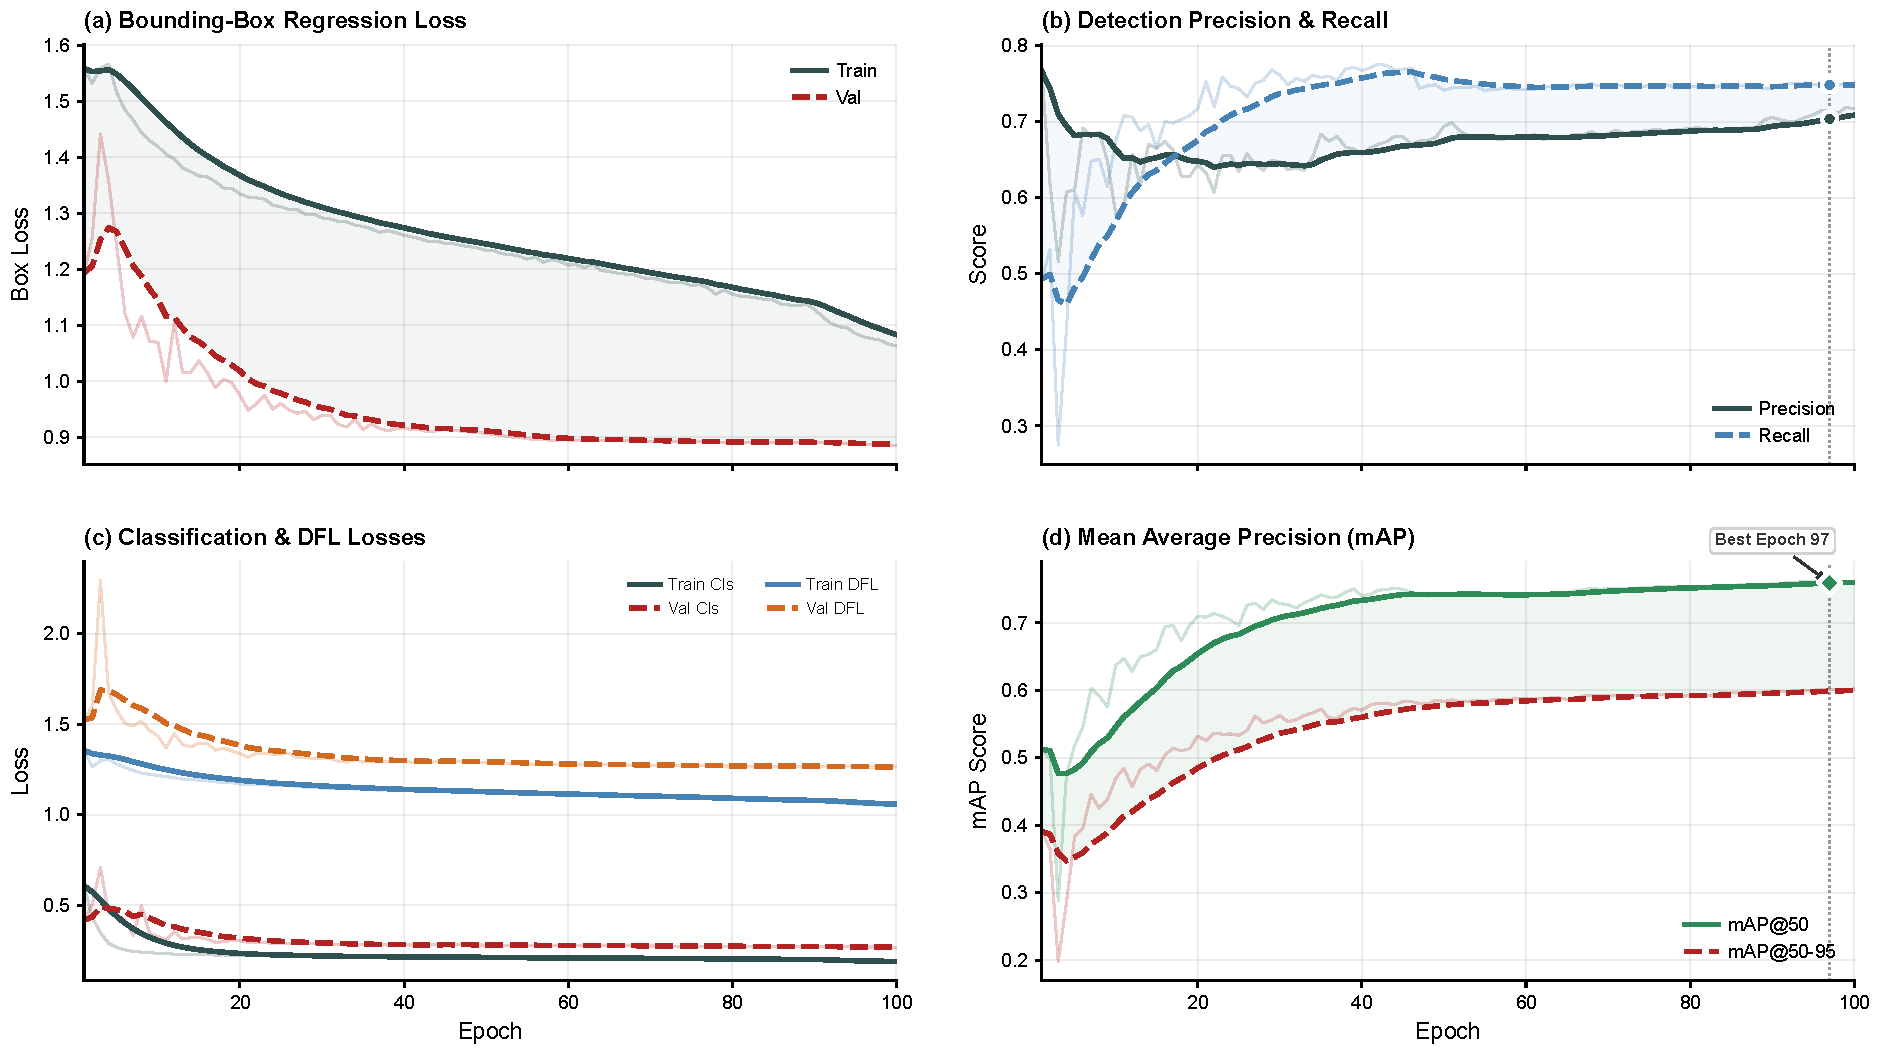
\includegraphics[height=0.4\textheight,keepaspectratio,width=\textwidth]{data/krishi_vaidya_yolo_data/outputs/figures/figure1_training_dynamics.pdf}
\caption{Training dynamics of the Krishi Vaidya YOLO detector}
\label{fig:yolo-training-dynamics}
\end{figure}

{\small \renewcommand{\arraystretch}{1.3}
\begin{xltabular}{\textwidth}{@{} l r @{}}
\caption{Summary of training dynamics and best-epoch performance for the YOLO detector}\label{tab:yolo-training-dynamics-summary}\\
\toprule
\textbf{Metric / Parameter} & \textbf{Value} \\
\midrule
\endfirsthead
\multicolumn{2}{l}{\textit{(continued from previous page)}} \\
\toprule
\textbf{Metric / Parameter} & \textbf{Value} \\
\midrule
\endhead
\midrule
\multicolumn{2}{r}{\textit{(continues on next page)}} \\
\endfoot
\bottomrule
\endlastfoot
Total epochs trained & $100$ \\
Best training epoch & $100$ \\
Input resolution (pixels) & $640 \times 640$ \\
Total training time & $7.12\,\text{hours}$ \\
\midrule
\multicolumn{2}{l}{\textit{Loss residuals at best epoch}} \\
Train box loss & $1.0627$ \\
Train class loss & $0.1871$ \\
Train DFL loss & $1.0493$ \\
Validation box loss & $0.8855$ \\
Validation class loss & $0.2681$ \\
Validation DFL loss & $1.2635$ \\
\midrule
\multicolumn{2}{l}{\textit{Detection accuracy at best epoch}} \\
Precision & $0.7172$ \\
Recall & $0.7487$ \\
F1-score & $0.7326$ \\
mAP@50 & $0.7616$ \\
mAP@50-95 & $0.6019$ \\
\end{xltabular}
}

Table~\ref{tab:yolo-training-dynamics-summary} reports the final metrics. Recall exceeds
precision, indicating that the detector favors object discovery over conservative filtering---a
useful property for a first-stage detector where missed plant regions cannot be analyzed
downstream. The gap between mAP@50 (0.7616) and mAP@50-95 (0.6019) reflects the difficulty of
precise localization under class imbalance and variable object scales.

\ChapterSubsection{YOLO Deployment and Threshold Results}

\subsubsection{Threshold Selection Behavior}

Figure~\ref{fig:yolo-threshold-sweep} and Table~\ref{tab:yolo-threshold-sensitivity-sweep}
present the confidence-threshold sweep. The highest F1-score (0.7362) occurs at threshold 0.10,
balancing precision of 0.7463 against recall of 0.7264. At the extremes, threshold 0.05
maximizes recall (0.7848) at the cost of precision, while 0.95 reduces recall to 0.0776 and
renders the detector ineffective.

\begin{figure}[H]
\centering
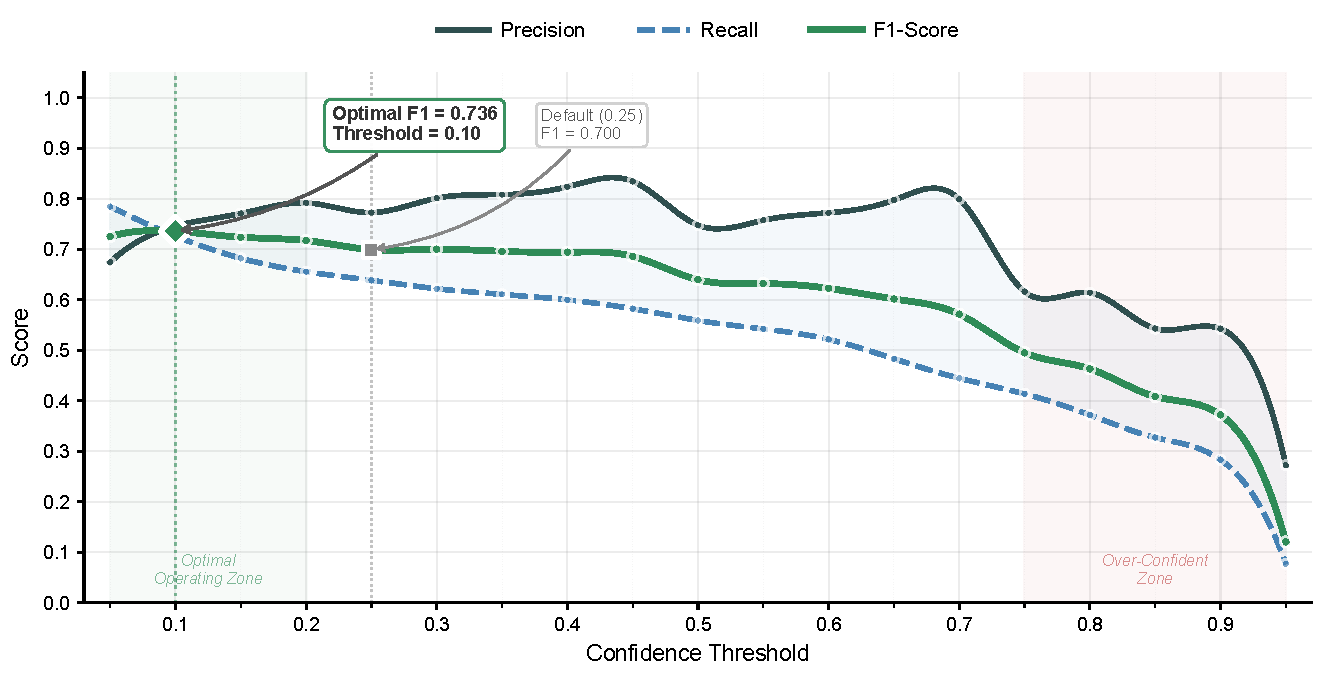
\includegraphics[height=0.5\textheight,keepaspectratio,width=\textwidth]{data/krishi_vaidya_yolo_data/outputs/figures/figure2_threshold_sweep.pdf}
\caption{Confidence-threshold sensitivity of the YOLO detector}
\label{fig:yolo-threshold-sweep}
\end{figure}

{\small  \renewcommand{\arraystretch}{1.3}
\begin{xltabular}{\textwidth}{@{} c c c c c c c @{}}
\caption{Sensitivity sweep of confidence thresholds on the YOLO baseline model}\label{tab:yolo-threshold-sensitivity-sweep}\\
\toprule
\textbf{Confidence threshold} & \textbf{Precision} & \textbf{Recall} & \textbf{F1-score} & \textbf{mAP@50} & \textbf{mAP@50-95} & \textbf{Fitness} \\
\midrule
\endfirsthead
\multicolumn{7}{l}{\textit{(continued from previous page)}} \\
\toprule
\textbf{Confidence threshold} & \textbf{Precision} & \textbf{Recall} & \textbf{F1-score} & \textbf{mAP@50} & \textbf{mAP@50-95} & \textbf{Fitness} \\
\midrule
\endhead
\midrule
\multicolumn{7}{r}{\textit{(continues on next page)}} \\
\endfoot
\bottomrule
\endlastfoot
0.05 & 0.6748 & 0.7848 & 0.7256 & 0.7225 & 0.5799 & 0.5799 \\
\textbf{0.10} & \textbf{0.7463} & \textbf{0.7264} & \textbf{0.7362} & \textbf{0.6879} & \textbf{0.5613} & \textbf{0.5613} \\
0.25 & 0.7729 & 0.6390 & 0.6996 & 0.6219 & 0.5227 & 0.5227 \\
0.40 & 0.8241 & 0.6003 & 0.6946 & 0.5885 & 0.4986 & 0.4986 \\
0.50 & 0.7480 & 0.5591 & 0.6399 & 0.5510 & 0.4712 & 0.4712 \\
0.75 & 0.6166 & 0.4140 & 0.4954 & 0.4109 & 0.3728 & 0.3728 \\
0.95 & 0.2727 & 0.0776 & 0.1208 & 0.0777 & 0.0729 & 0.0729 \\
\end{xltabular}
}

\subsubsection{Quantization Tradeoffs}

Figure~\ref{fig:yolo-quantization-comparison} and Table~\ref{tab:yolo-deployment-efficiency}
compare the baseline PyTorch model against three TFLite variants. The baseline runs at 12.18 ms
per image (82.1 FPS) on cuda:0. INT8 achieves the strongest compression (1.87$\times$, 3.20 MB)
but drops F1 to 0.7268. FP16 preserves performance more closely (F1 of 0.7377) at 5.90 MB.
Final deployment selection requires on-device Android profiling, as the reported latencies
reflect GPU measurements.

\begin{figure}[H]
\centering
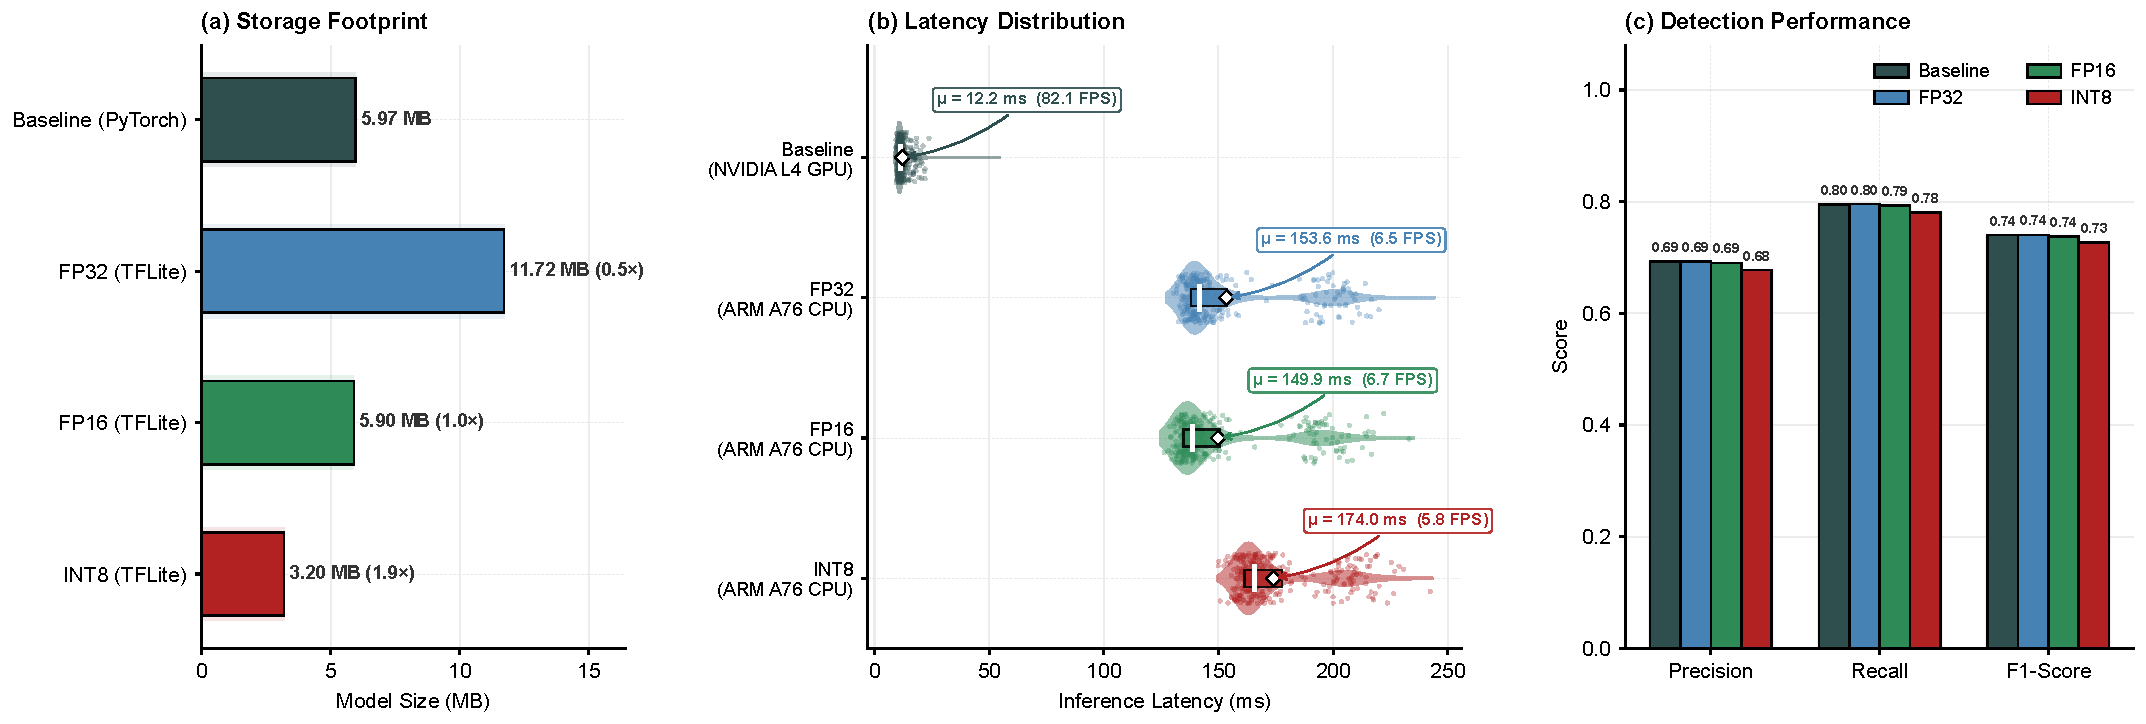
\includegraphics[height=0.6\textheight,keepaspectratio,width=\textwidth]{data/krishi_vaidya_yolo_data/outputs/figures/figure3_quantization_comparison.pdf}
\caption{Deployment comparison across baseline and quantized YOLO variants}
\label{fig:yolo-quantization-comparison}
\end{figure}

{\scriptsize \renewcommand{\arraystretch}{1.3}
\begin{xltabular}{\textwidth}{@{} l c c c c c c c c @{}}
\caption{Deployment efficiency comparison across YOLO model variants}\label{tab:yolo-deployment-efficiency}\\
\toprule
\textbf{Variant} & \textbf{Size (MB)} & \textbf{Compression} & \textbf{Device} & \textbf{Latency (ms)} & \textbf{FPS} & \textbf{Precision} & \textbf{Recall} & \textbf{F1} \\
\midrule
\endfirsthead
\multicolumn{9}{l}{\textit{(continued from previous page)}} \\
\toprule
\textbf{Variant} & \textbf{Size (MB)} & \textbf{Compression} & \textbf{Device} & \textbf{Latency (ms)} & \textbf{FPS} & \textbf{Precision} & \textbf{Recall} & \textbf{F1} \\
\midrule
\endhead
\midrule
\multicolumn{9}{r}{\textit{(continues on next page)}} \\
\endfoot
\bottomrule
\endlastfoot
Baseline (PyTorch) & 5.97 & 1.00$\times$ & cuda:0 & 12.18 & 82.1 & 0.6929 & 0.7952 & 0.7402 \\
FP32 (TFLite) & 11.72 & 0.51$\times$ & cuda:0 & 153.59 & 6.5 & 0.6930 & 0.7957 & 0.7402 \\
FP16 (TFLite) & 5.90 & 1.01$\times$ & cuda:0 & 149.94 & 6.7 & 0.6903 & 0.7926 & 0.7377 \\
INT8 (TFLite) & 3.20 & 1.87$\times$ & cuda:0 & 174.01 & 5.8 & 0.6774 & 0.7811 & 0.7268 \\
\end{xltabular}
}

\subsubsection{Per-Class Behavior}

Table~\ref{tab:yolo-per-class-f1-comparison} reveals that quantization impacts classes unevenly.
The optimal format varies by class: baseline PyTorch excels for rice leaf, rice panicle, tomato
leaf, brassica leaf, and cabbage head, while FP32 favors rice grain cluster and tomato fruit,
FP16 benefits potato leaf, and INT8 performs best for maize leaf and cauliflower head. Deployment
strategies must therefore consider the specific classes most critical to the target use case.

{\small \renewcommand{\arraystretch}{1.3}
\begin{xltabular}{\textwidth}{@{} l c c c c @{}}
\caption{Per-class F1-score comparison across YOLO model variants}\label{tab:yolo-per-class-f1-comparison}\\
\toprule
\textbf{Class} & \textbf{Baseline (PyTorch)} & \textbf{FP32 (TFLite)} & \textbf{FP16 (TFLite)} & \textbf{INT8 (TFLite)} \\
\midrule
\endfirsthead
\multicolumn{5}{l}{\textit{(continued from previous page)}} \\
\toprule
\textbf{Class} & \textbf{Baseline (PyTorch)} & \textbf{FP32 (TFLite)} & \textbf{FP16 (TFLite)} & \textbf{INT8 (TFLite)} \\
\midrule
\endhead
\midrule
\multicolumn{5}{r}{\textit{(continues on next page)}} \\
\endfoot
\bottomrule
\endlastfoot
Rice leaf & \textbf{0.7750} & 0.7716 & 0.7207 & 0.7124 \\
Rice panicle & \textbf{0.7799} & 0.7295 & 0.7277 & 0.7426 \\
Rice grain cluster & 0.6911 & \textbf{0.7563} & 0.6980 & 0.7093 \\
Maize leaf & 0.7139 & 0.7162 & 0.7137 & \textbf{0.7655} \\
Maize ear & 0.6934 & \textbf{0.7736} & 0.7115 & 0.7363 \\
Potato leaf & 0.7446 & 0.7219 & \textbf{0.7857} & 0.6977 \\
Tomato leaf & \textbf{0.7793} & 0.7089 & 0.7336 & 0.6885 \\
Tomato fruit & 0.7788 & \textbf{0.7852} & 0.7085 & 0.7083 \\
Brassica leaf & \textbf{0.7876} & 0.7327 & 0.7240 & 0.7118 \\
Cauliflower head & 0.7164 & 0.7058 & 0.7255 & \textbf{0.7361} \\
Cabbage head & \textbf{0.7833} & 0.7252 & 0.7740 & 0.7245 \\
\end{xltabular}
}

\ChapterSubsection{YOLO Error Analysis}


\subsubsection{Error Categories}

Table~\ref{tab:yolo-error-analysis} breaks down true positives, missed detections, and ghost
detections by class. Rice panicle dominates the failure profile: 16,147 objects missed (92.9\%
false negatives). Rice leaf also has a 98.0\% miss rate, and brassica leaf records zero true
positives. In contrast, maize leaf and tomato leaf show strong performance with missed-detection
rates below 1\%.

{\small \renewcommand{\arraystretch}{1.3}
\begin{xltabular}{\textwidth}{@{} l r r r @{}}
\caption{Error analysis breakdown by YOLO class}\label{tab:yolo-error-analysis}\\
\toprule
\textbf{Class} & \textbf{True positives} & \textbf{False negatives (missed)} & \textbf{False positives (ghost)} \\
\midrule
\endfirsthead
\multicolumn{4}{l}{\textit{(continued from previous page)}} \\
\toprule
\textbf{Class} & \textbf{True positives} & \textbf{False negatives (missed)} & \textbf{False positives (ghost)} \\
\midrule
\endhead
\midrule
\multicolumn{4}{r}{\textit{(continues on next page)}} \\
\endfoot
\bottomrule
\endlastfoot
\textbf{Rice panicle} & 1,238 & 16,147 (92.9\%) & 46 (3.6\%) \\
Rice leaf & 7 & 339 (98.0\%) & 4 (36.4\%) \\
Tomato fruit & 168 & 119 (41.5\%) & 9 (5.1\%) \\
Rice grain cluster & 58 & 24 (29.3\%) & 68 (54.0\%) \\
Brassica leaf & 0 & 75 (100.0\%) & 0 (0.0\%) \\
Potato leaf & 129 & 19 (12.8\%) & 23 (15.1\%) \\
Maize leaf & 990 & 10 (1.0\%) & 11 (1.1\%) \\
Tomato leaf & 1,039 & 8 (0.8\%) & 4 (0.4\%) \\
Maize ear & 3 & 1 (25.0\%) & 4 (57.1\%) \\
Cabbage head & 45 & 0 (0.0\%) & 2 (4.3\%) \\
Cauliflower head & 24 & 0 (0.0\%) & 0 (0.0\%) \\
\end{xltabular}
}

The rice panicle result warrants careful interpretation. Although 115,046 annotations dominate
the class distribution, these objects are small, clustered, and visually dense. Consistent with
findings in agricultural small-object detection literature \parencite{zhengSmallObjDetAgri2023},
lightweight YOLO architectures struggle to preserve spatial detail for dense fine structures.
Improving this class will likely require targeted data review, higher-resolution training, and
augmentation strategies designed for small clustered objects.


\subsubsection{Summary of YOLO Findings}

The YOLO detector achieved F1 of 0.7326, mAP@50 of 0.7616, and mAP@50-95 of 0.6019.
The threshold sweep identifies 0.10 as the best F1 operating point. TFLite variants preserve
useful performance, with INT8 providing the smallest footprint and FP16 offering a closer
accuracy--size compromise. The main limitation is class-specific reliability: the detector
handles some classes well but struggles with dense or underrepresented structures. Its outputs
are best treated as supporting evidence for downstream diagnosis rather than standalone
disease labels.
\subsubsection{Confusion Patterns}

Figure~\ref{fig:yolo-confusion-matrix} presents the confusion matrix, which exposes whether
failures concentrate in a few classes---a pattern that aggregate metrics alone cannot reveal
under severe class imbalance.

\begin{figure}[H]
\centering
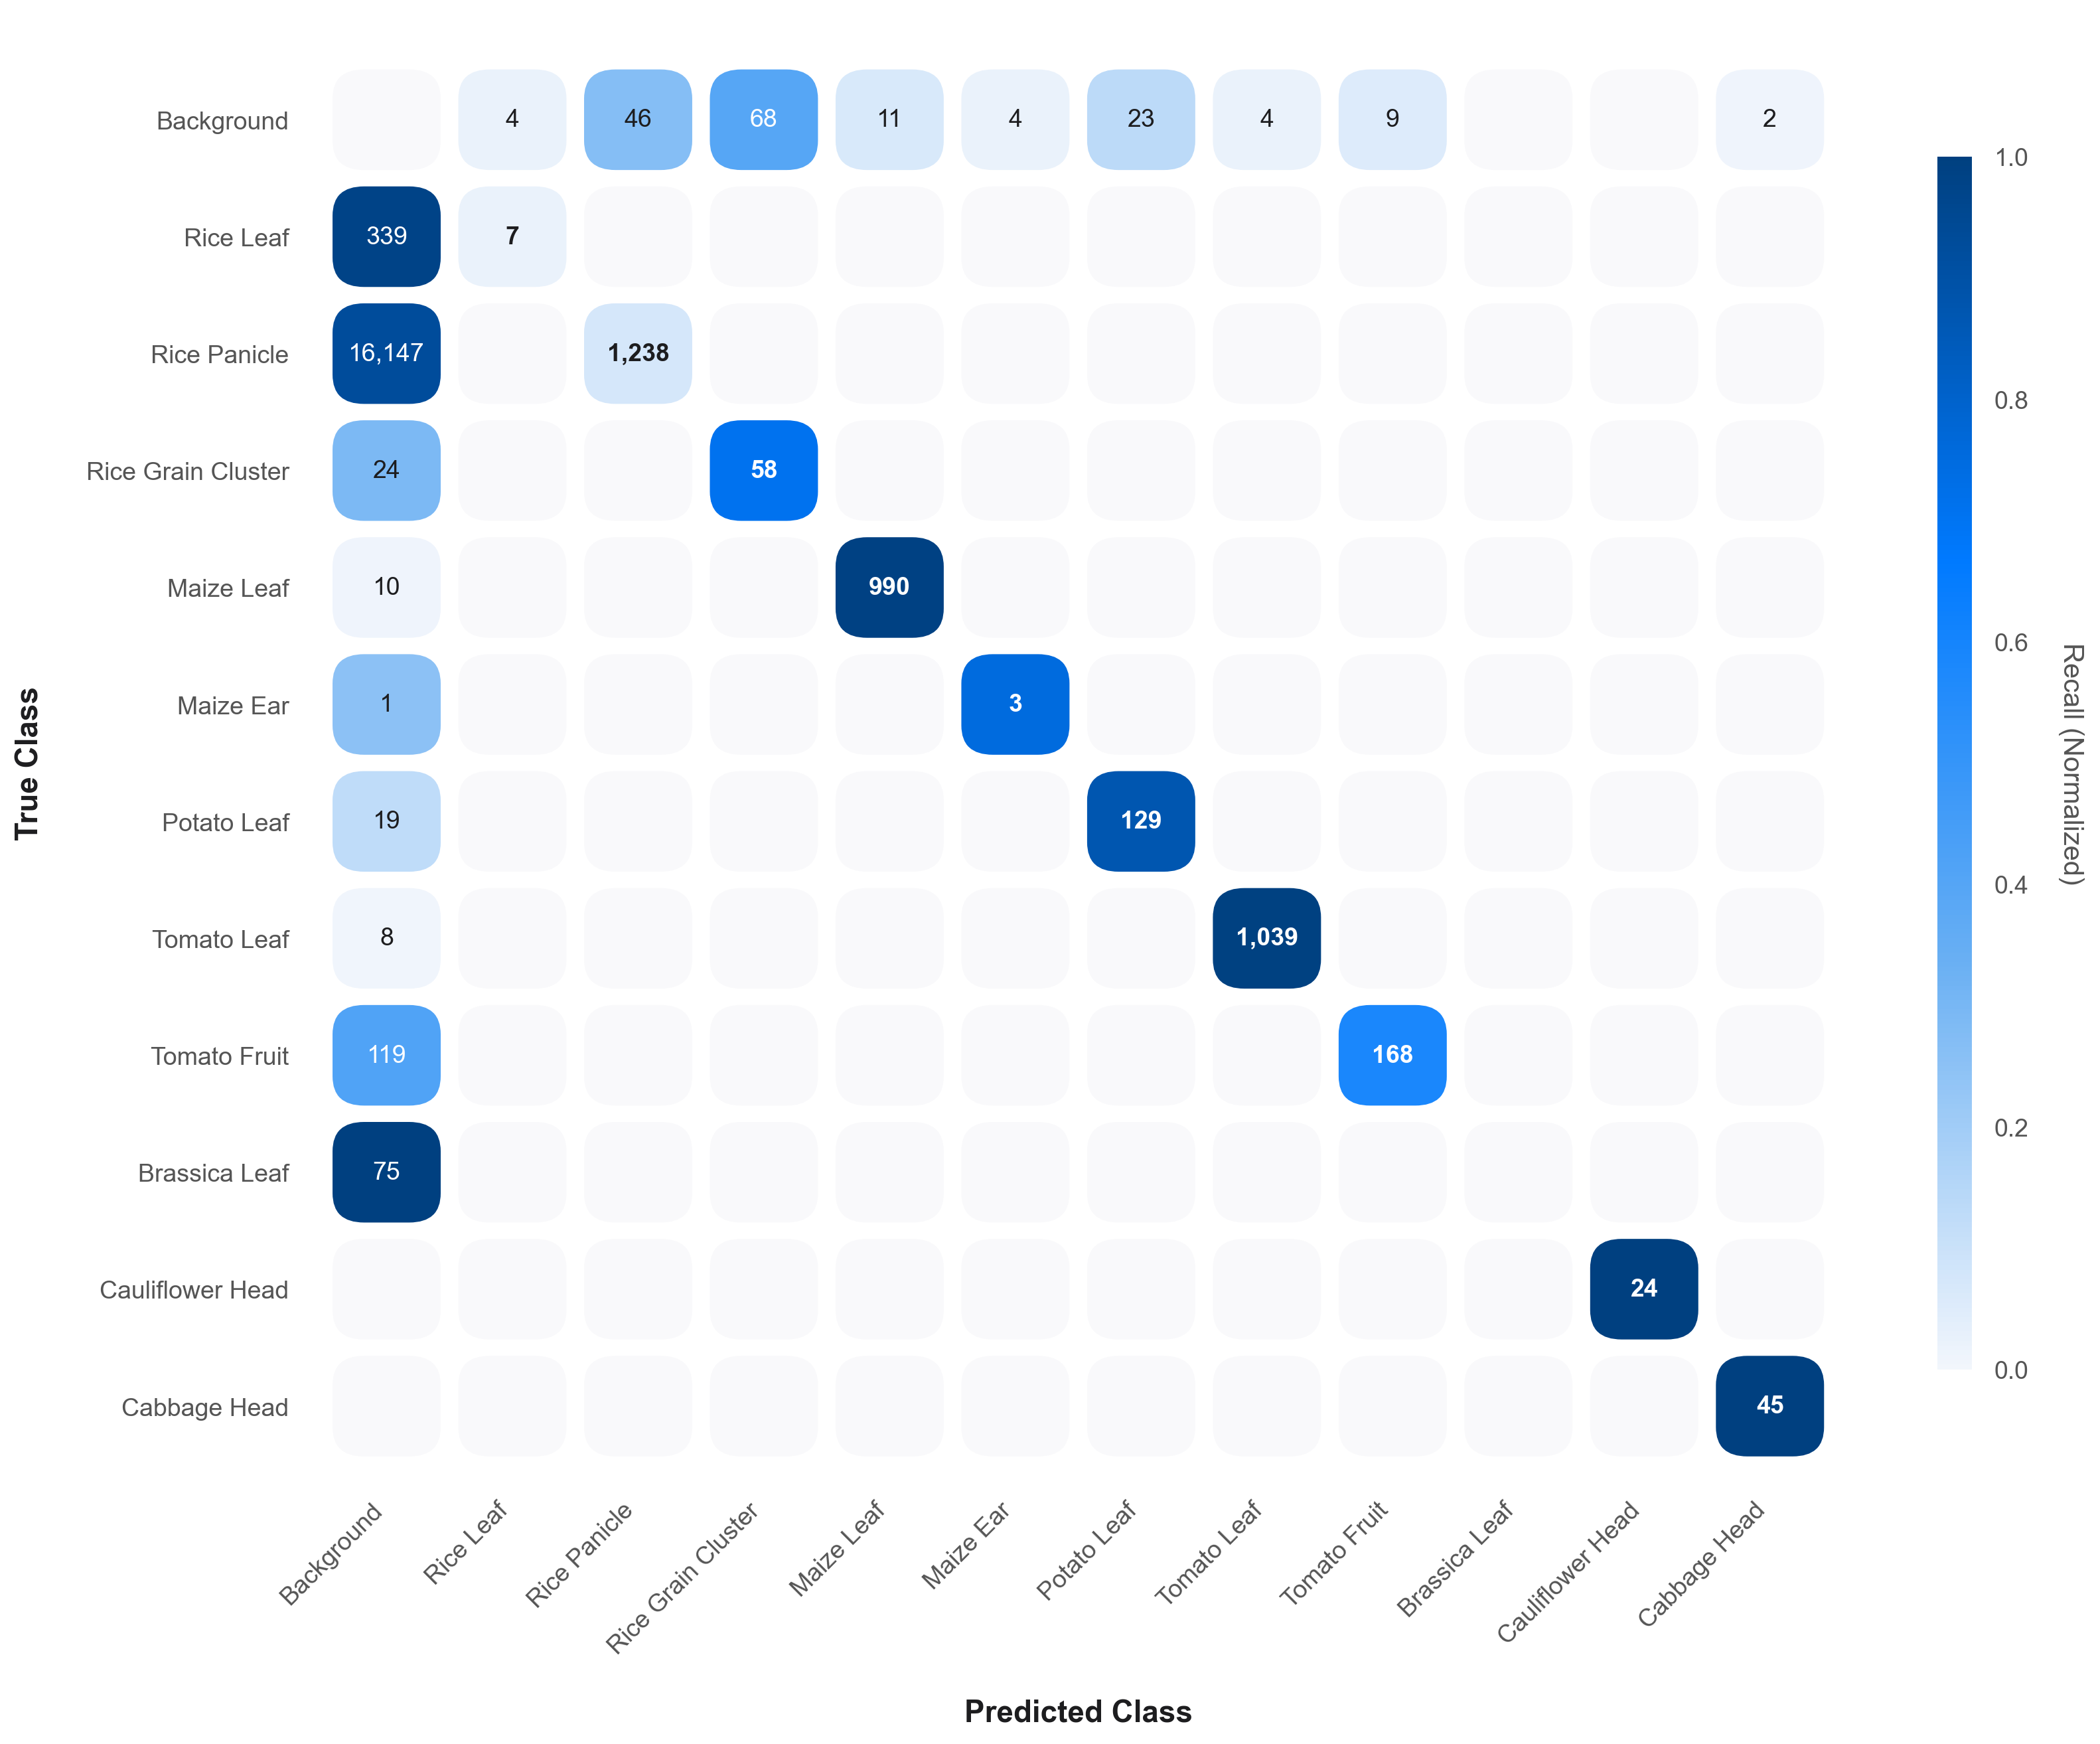
\includegraphics[height=0.6\textheight,keepaspectratio,width=0.92\textwidth]{data/krishi_vaidya_yolo_data/outputs/figures/figure4_confusion_matrix.png}
\caption{Confusion matrix of the YOLO detector}
\label{fig:yolo-confusion-matrix}
\end{figure}
\ChapterSubsection{VLM Training and Resource Results}

\subsubsection{Fine-Tuning Performance}

The VLM completed 3 epochs and 969 training steps using Qwen2.5-VL-3B-Instruct as the base
model. Figure~\ref{fig:vlm-training-dynamics} shows the training trajectory, and
Table~\ref{tab:vlm-training-summary} reports the outcome. The final evaluation loss is 0.0146
with mean token accuracy of 0.9967, confirming that the model learned the supervised answer
format. However, low evaluation loss does not guarantee parseable or correct disease labels
during free generation; the prediction study in
Section~\ref{sec:vlm-prediction-results} evaluates that separately.



{\small \renewcommand{\arraystretch}{1.3}
\begin{xltabular}{\textwidth}{@{} l r @{}}
\caption{Training summary for Qwen2.5-VL LoRA fine-tuning}\label{tab:vlm-training-summary}\\
\toprule
\textbf{Metric / setting} & \textbf{Value} \\
\midrule
\endfirsthead
\multicolumn{2}{l}{\textit{(continued from previous page)}} \\
\toprule
\textbf{Metric / setting} & \textbf{Value} \\
\midrule
\endhead
\midrule
\multicolumn{2}{r}{\textit{(continues on next page)}} \\
\endfoot
\bottomrule
\endlastfoot
Base model & Qwen/Qwen2.5-VL-3B-Instruct \\
Epochs completed & 3.00 \\
Train steps & 969 \\
Last logged train loss & 0.0097 \\
Trainer-reported train loss & 0.1048 \\
Final eval loss & 0.0146 \\
Mean token accuracy & 0.9967 \\
Runtime & 2.58 h \\
Samples/sec & 1.664 \\
Learning rate & 2.00e-05 \\
Effective batch & 4 x 4 \\
LoRA rank / alpha & 16 / 32 \\
Quantization & 4-bit nf4 \\
\end{xltabular}
}
\begin{figure}[H]
\centering
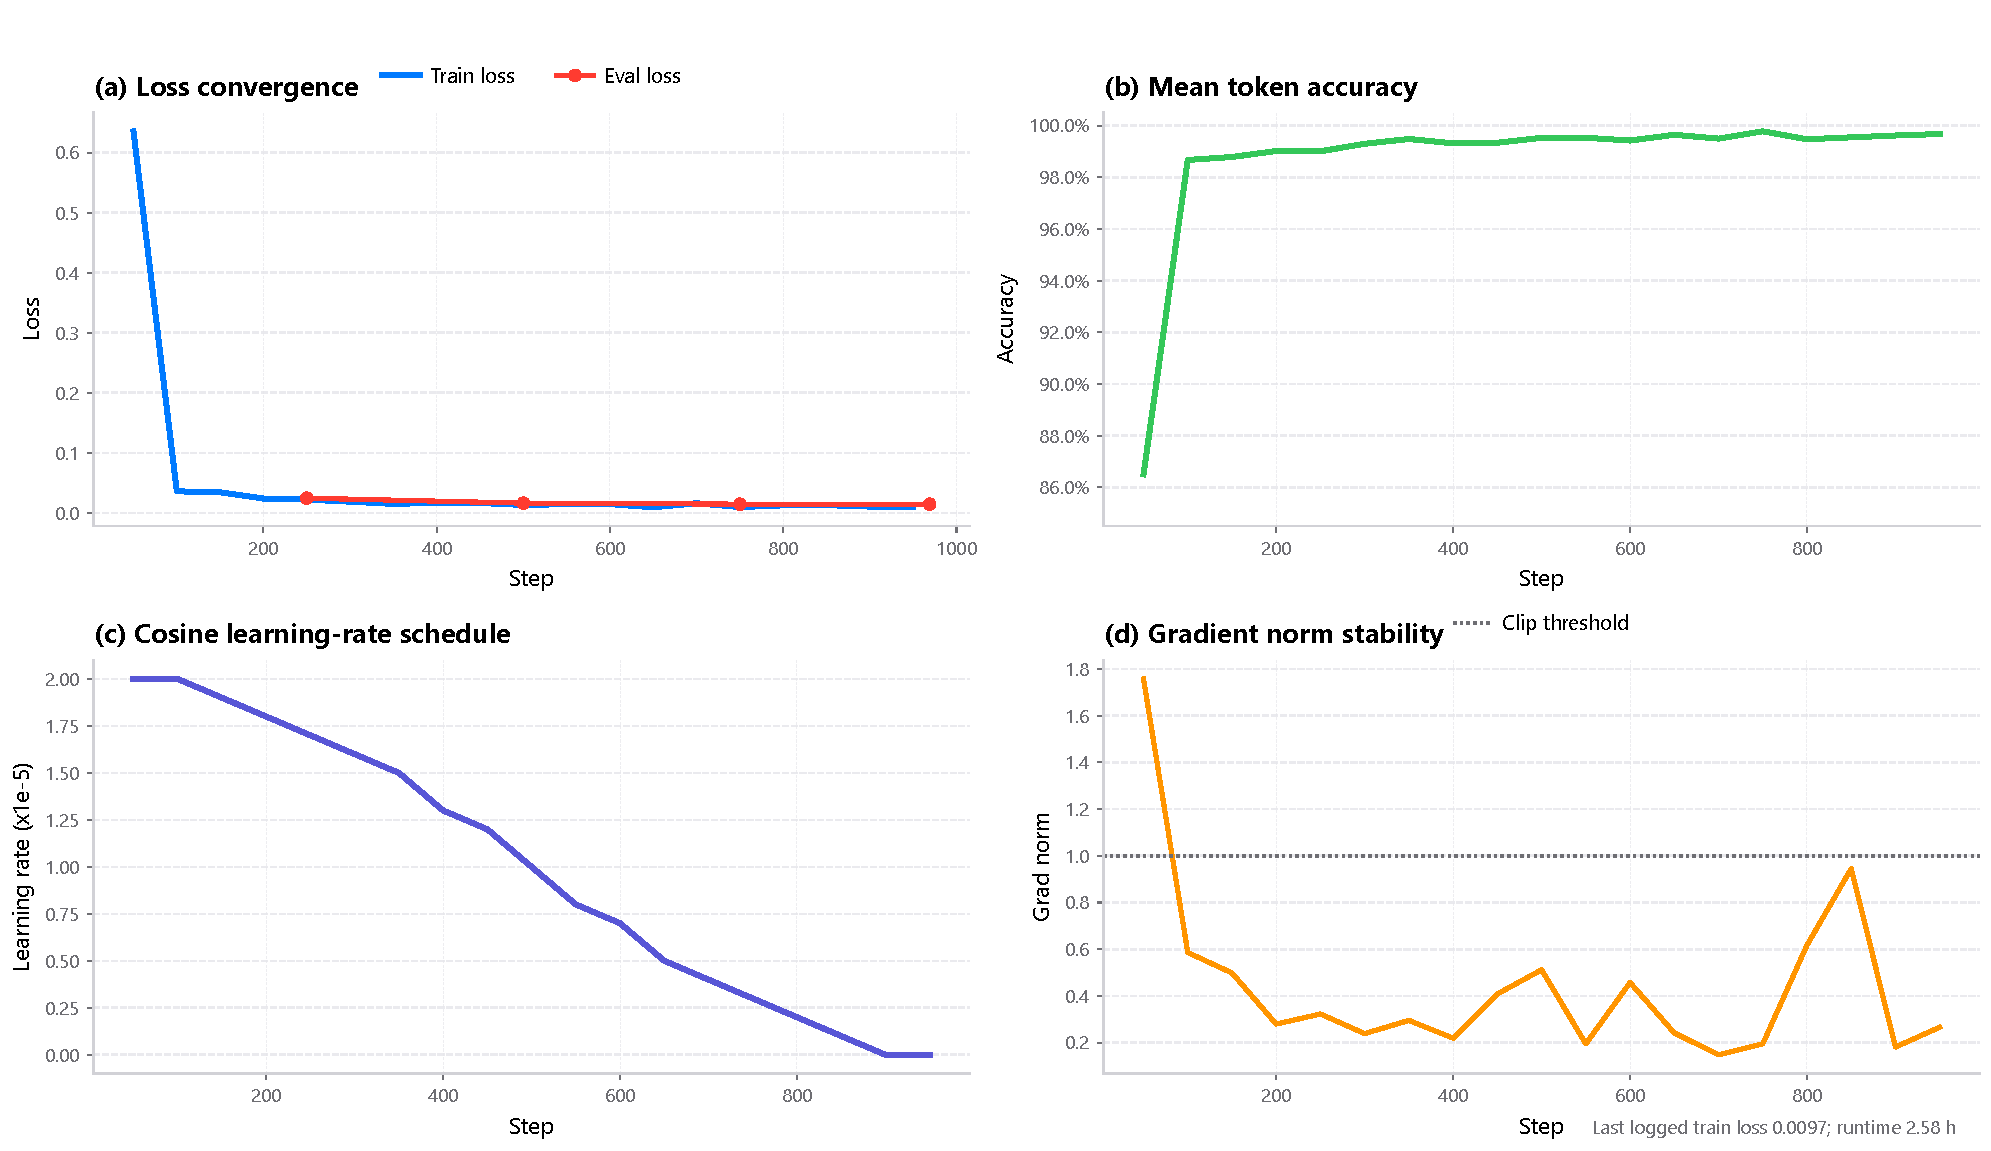
\includegraphics[height=0.45\textheight,keepaspectratio,width=\textwidth]{data/krishi_vaidya_vlm_data/outputs/figures/figure1_training_dynamics.pdf}
\caption{Training dynamics of the Qwen2.5-VL LoRA fine-tuning run}
\label{fig:vlm-training-dynamics}
\end{figure}
\subsubsection{Runtime and Memory Behavior}

Training ran on an NVIDIA L4 GPU (CUDA 12.8, compute capability 8.9) with
\texttt{flash\_attention\_2}, Liger kernel, bfloat16, and TF32 enabled. Peak allocated GPU
memory reached 12.56 GB of the available 22.03 GB, and peak reserved memory was 13.08 GB.
Figure~\ref{fig:vlm-memory-runtime} shows the resource profile, confirming feasibility of
adapter fine-tuning a 3B-parameter VLM under a single-GPU setup with 4-bit NF4 quantization.

\begin{figure}[H]
\centering
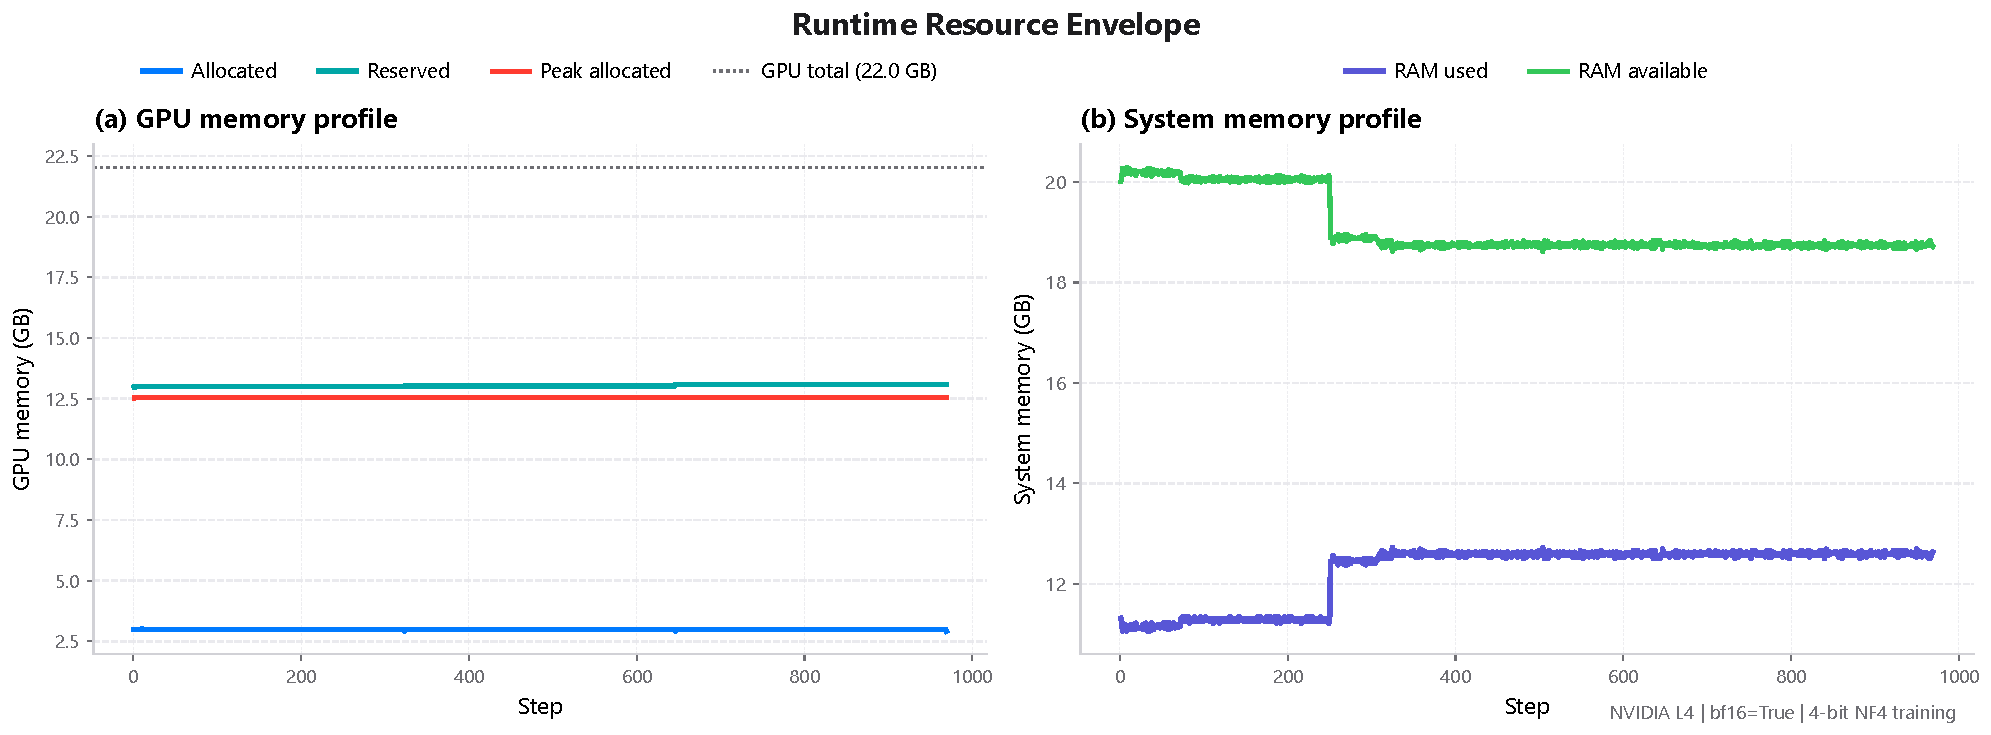
\includegraphics[height=0.4\textheight,keepaspectratio,width=\textwidth]{data/krishi_vaidya_vlm_data/outputs/figures/figure2_memory_runtime.pdf}
\caption{Runtime and memory behavior of the VLM training run}
\label{fig:vlm-memory-runtime}
\end{figure}

\ChapterSubsection{VLM Prediction Results}
\label{sec:vlm-prediction-results}

\subsubsection{Dataset Split and Class Distribution}

Table~\ref{tab:vlm-dataset-splits} summarizes the Qwen export: 6,647 records across train
(5,147), validation (702), and test (798) splits, with image counts exactly twice the record
counts per split. The class distribution is partially capped but uneven---several classes
contain 800 records while potato healthy contains only 72. In the test split, maize common rust
alone contributes 412 of 798 examples, making the model's behavior on that class especially
important for the aggregate accuracy.
Figure~\ref{fig:vlm-dataset-composition} visualizes the composition.

{\small \renewcommand{\arraystretch}{1.3}
\begin{xltabular}{\textwidth}{@{} l r r @{}}
\caption{Dataset split validation summary for VLM records}\label{tab:vlm-dataset-splits}\\
\toprule
\textbf{Split} & \textbf{Qwen records} & \textbf{Images found} \\
\midrule
\endfirsthead
\multicolumn{3}{l}{\textit{(continued from previous page)}} \\
\toprule
\textbf{Split} & \textbf{Qwen records} & \textbf{Images found} \\
\midrule
\endhead
\midrule
\multicolumn{3}{r}{\textit{(continues on next page)}} \\
\endfoot
\bottomrule
\endlastfoot
Train & 5,147 & 10,294 \\
Validation & 702 & 1,404 \\
Test & 798 & 1,596 \\
Total & 6,647 & 13,294 \\
\end{xltabular}
}

\begin{figure}[H]
\centering
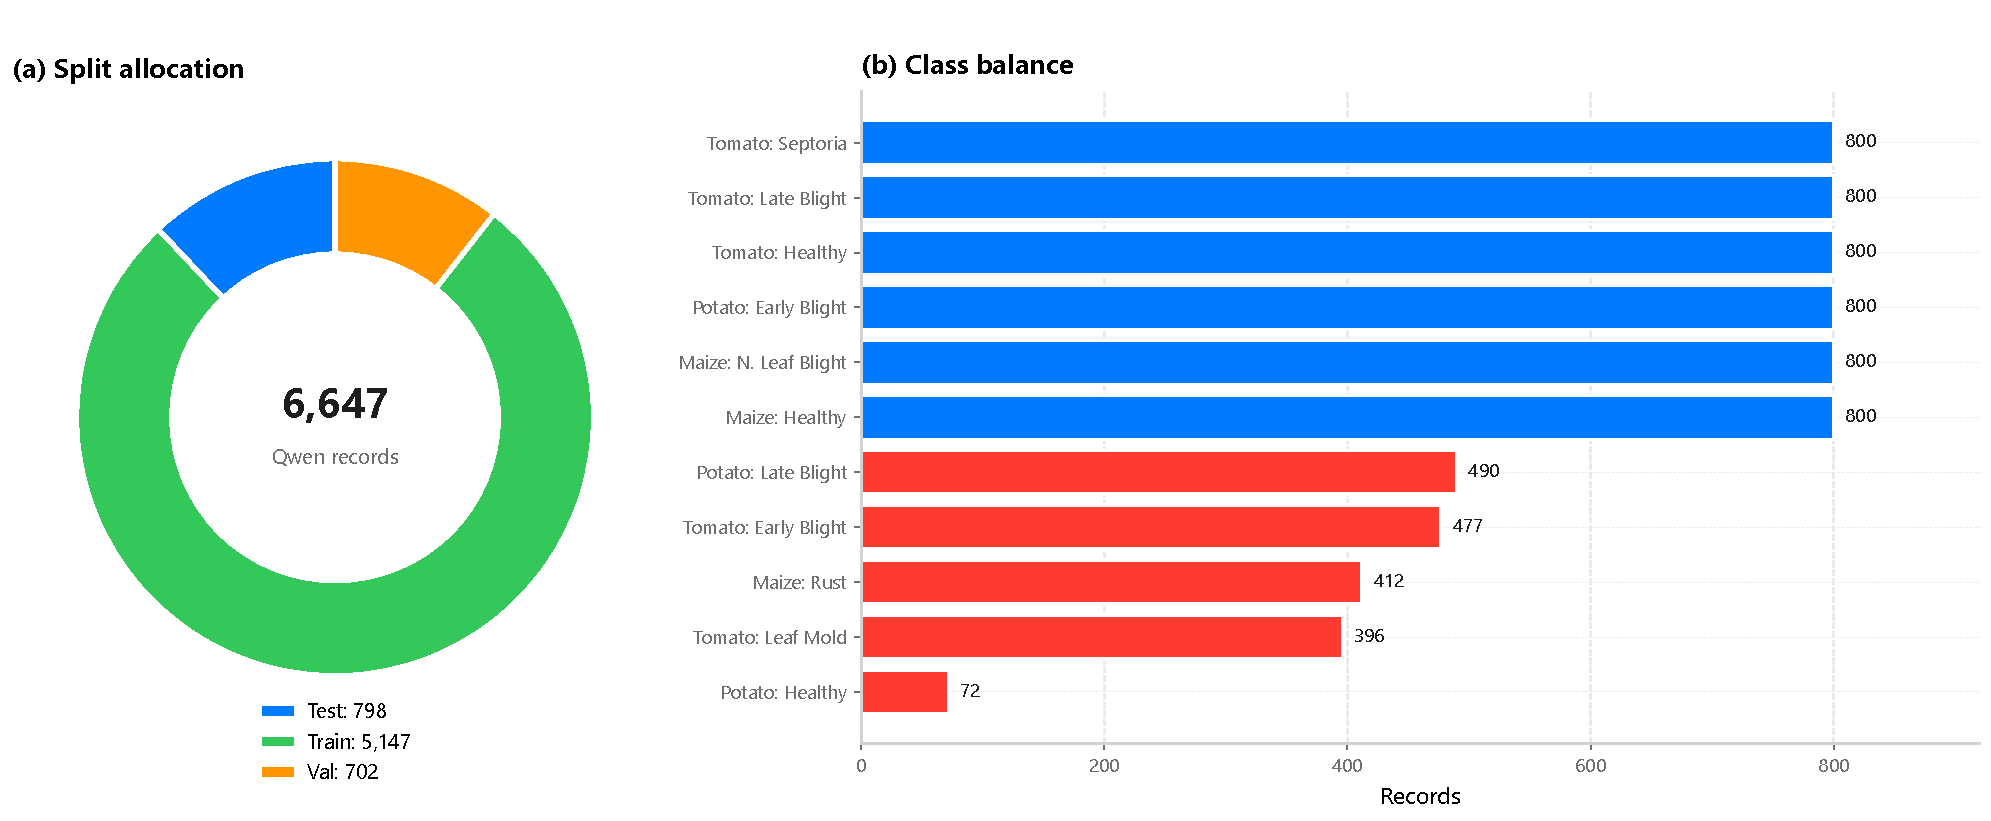
\includegraphics[height=0.4\textheight,keepaspectratio,width=\textwidth]{data/krishi_vaidya_vlm_data/outputs/figures/figure3_dataset_composition.pdf}
\caption{Dataset composition for the VLM Qwen export}
\label{fig:vlm-dataset-composition}
\end{figure}

\subsubsection{Prediction Summary}

Table~\ref{tab:vlm-prediction-summary} reports test-set prediction metrics: accuracy of 0.1303,
macro precision of 0.5232, macro recall of 0.1834, and macro F1 of 0.2465. The dominant
constraint is parseability---540 of 798 predictions (67.7\%) failed to produce an extractable
\texttt{canonical\_label} and were recorded as parse errors.
Figure~\ref{fig:vlm-prediction-performance} visualizes the performance breakdown.

\begin{figure}[H]
\centering
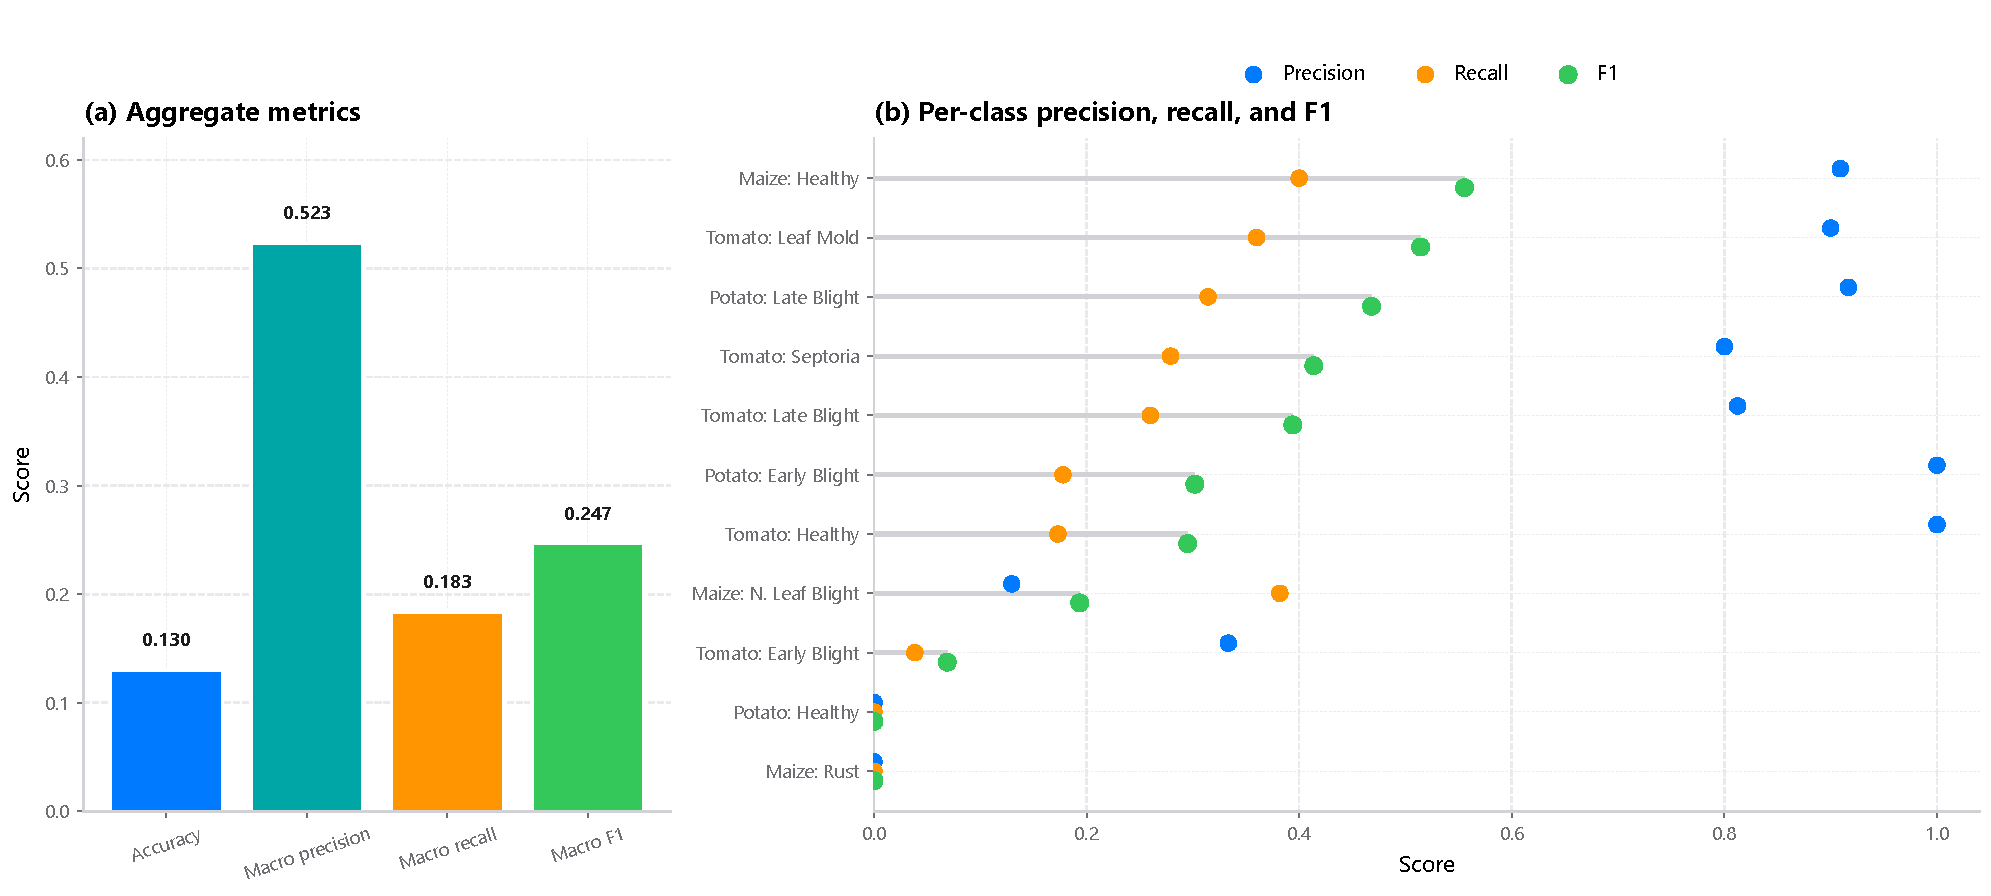
\includegraphics[height=0.4\textheight,keepaspectratio,width=\textwidth]{data/krishi_vaidya_vlm_data/outputs/figures/figure4_prediction_performance.pdf}
\caption{Prediction performance of the VLM on the test split}
\label{fig:vlm-prediction-performance}
\end{figure}

{\small \renewcommand{\arraystretch}{1.3}
\begin{xltabular}{\textwidth}{@{} l r @{}}
\caption{Prediction summary on the VLM test split}\label{tab:vlm-prediction-summary}\\
\toprule
\textbf{Metric} & \textbf{Value} \\
\midrule
\endfirsthead
\multicolumn{2}{l}{\textit{(continued from previous page)}} \\
\toprule
\textbf{Metric} & \textbf{Value} \\
\midrule
\endhead
\midrule
\multicolumn{2}{r}{\textit{(continues on next page)}} \\
\endfoot
\bottomrule
\endlastfoot
Split & test \\
Examples & 798 \\
Accuracy & 0.1303 \\
Macro precision & 0.5232 \\
Macro recall & 0.1834 \\
Macro F1 & 0.2465 \\
Parse-error predictions & 540 (67.7\%) \\
\end{xltabular}
}

The high parse-error rate likely reflects interacting factors: the small 3B-parameter base,
LoRA-only adaptation, a three-epoch budget, online-source dataset variability, mixed prompt
templates, and unconstrained autoregressive decoding. Future iterations should pair lightweight
VLMs with longer training, stricter decoding, stronger format supervision, or post-generation
repair \parencite{paleyes2022MLSystemsChallenges}.

\subsubsection{Per-Class Prediction Metrics}

Table~\ref{tab:vlm-per-class-metrics} shows uneven per-class behavior. Maize healthy obtains
the highest F1 at 0.5556, followed by tomato leaf mold (0.5143), potato late blight (0.4681),
tomato septoria leaf spot (0.4138), and tomato late blight (0.3939). Several classes perform
poorly: maize common rust has 412 false negatives and zero true positives, potato healthy has no
true positives, and tomato early blight has only one. The model also emits one prediction for
maize early leaf spot---a label outside the supported class set---indicating that output
constraints are needed to prevent out-of-vocabulary generation.

{\small \renewcommand{\arraystretch}{1.3}
\begin{xltabular}{\textwidth}{@{} l r r r r r r r @{}}
\caption{Per-class prediction metrics for the VLM test split}\label{tab:vlm-per-class-metrics}\\
\toprule
\textbf{Class} & \textbf{Support} & \textbf{Precision} & \textbf{Recall} & \textbf{F1} & \textbf{TP} & \textbf{FN} & \textbf{FP} \\
\midrule
\endfirsthead
\multicolumn{8}{l}{\textit{(continued from previous page)}} \\
\toprule
\textbf{Class} & \textbf{Support} & \textbf{Precision} & \textbf{Recall} & \textbf{F1} & \textbf{TP} & \textbf{FN} & \textbf{FP} \\
\midrule
\endhead
\midrule
\multicolumn{8}{r}{\textit{(continues on next page)}} \\
\endfoot
\bottomrule
\endlastfoot
Maize: Common Rust & 412 & 0.0000 & 0.0000 & 0.0000 & 0 & 412 & 0 \\
Maize: Healthy & 50 & 0.9091 & 0.4000 & 0.5556 & 20 & 30 & 2 \\
Maize: Northern Leaf Blight & 55 & 0.1296 & 0.3818 & 0.1935 & 21 & 34 & 141 \\
Potato: Early Blight & 45 & 1.0000 & 0.1778 & 0.3019 & 8 & 37 & 0 \\
Potato: Healthy & 5 & 0.0000 & 0.0000 & 0.0000 & 0 & 5 & 0 \\
Potato: Late Blight & 35 & 0.9167 & 0.3143 & 0.4681 & 11 & 24 & 1 \\
Tomato: Early Blight & 26 & 0.3333 & 0.0385 & 0.0690 & 1 & 25 & 2 \\
Tomato: Healthy & 52 & 1.0000 & 0.1731 & 0.2951 & 9 & 43 & 0 \\
Tomato: Late Blight & 50 & 0.8125 & 0.2600 & 0.3939 & 13 & 37 & 3 \\
Tomato: Leaf Mold & 25 & 0.9000 & 0.3600 & 0.5143 & 9 & 16 & 1 \\
Tomato: Septoria Leaf Spot & 43 & 0.8000 & 0.2791 & 0.4138 & 12 & 31 & 3 \\
Parse Error & 0 & 0.0000 & 0.0000 & 0.0000 & 0 & 0 & 540 \\
Maize: Early Leaf Spot & 0 & 0.0000 & 0.0000 & 0.0000 & 0 & 0 & 1 \\
\end{xltabular}
}

\subsubsection{Confusion Matrix and Prediction Distribution}

Figures~\ref{fig:vlm-confusion-matrix} and~\ref{fig:vlm-inference-diagnostics} visualize
prediction distribution and diagnostic patterns. The dominant parse-error column confirms that
the primary constraint is not inter-class confusion but the difficulty of producing parseable
canonical answers under the current training and decoding setup. Parse-error predictions also
carry higher median latency (7.32 s) than successful labels (5.32--6.67 s), suggesting that
output-format constraints would improve both accuracy and throughput.

\begin{figure}[H]
\centering
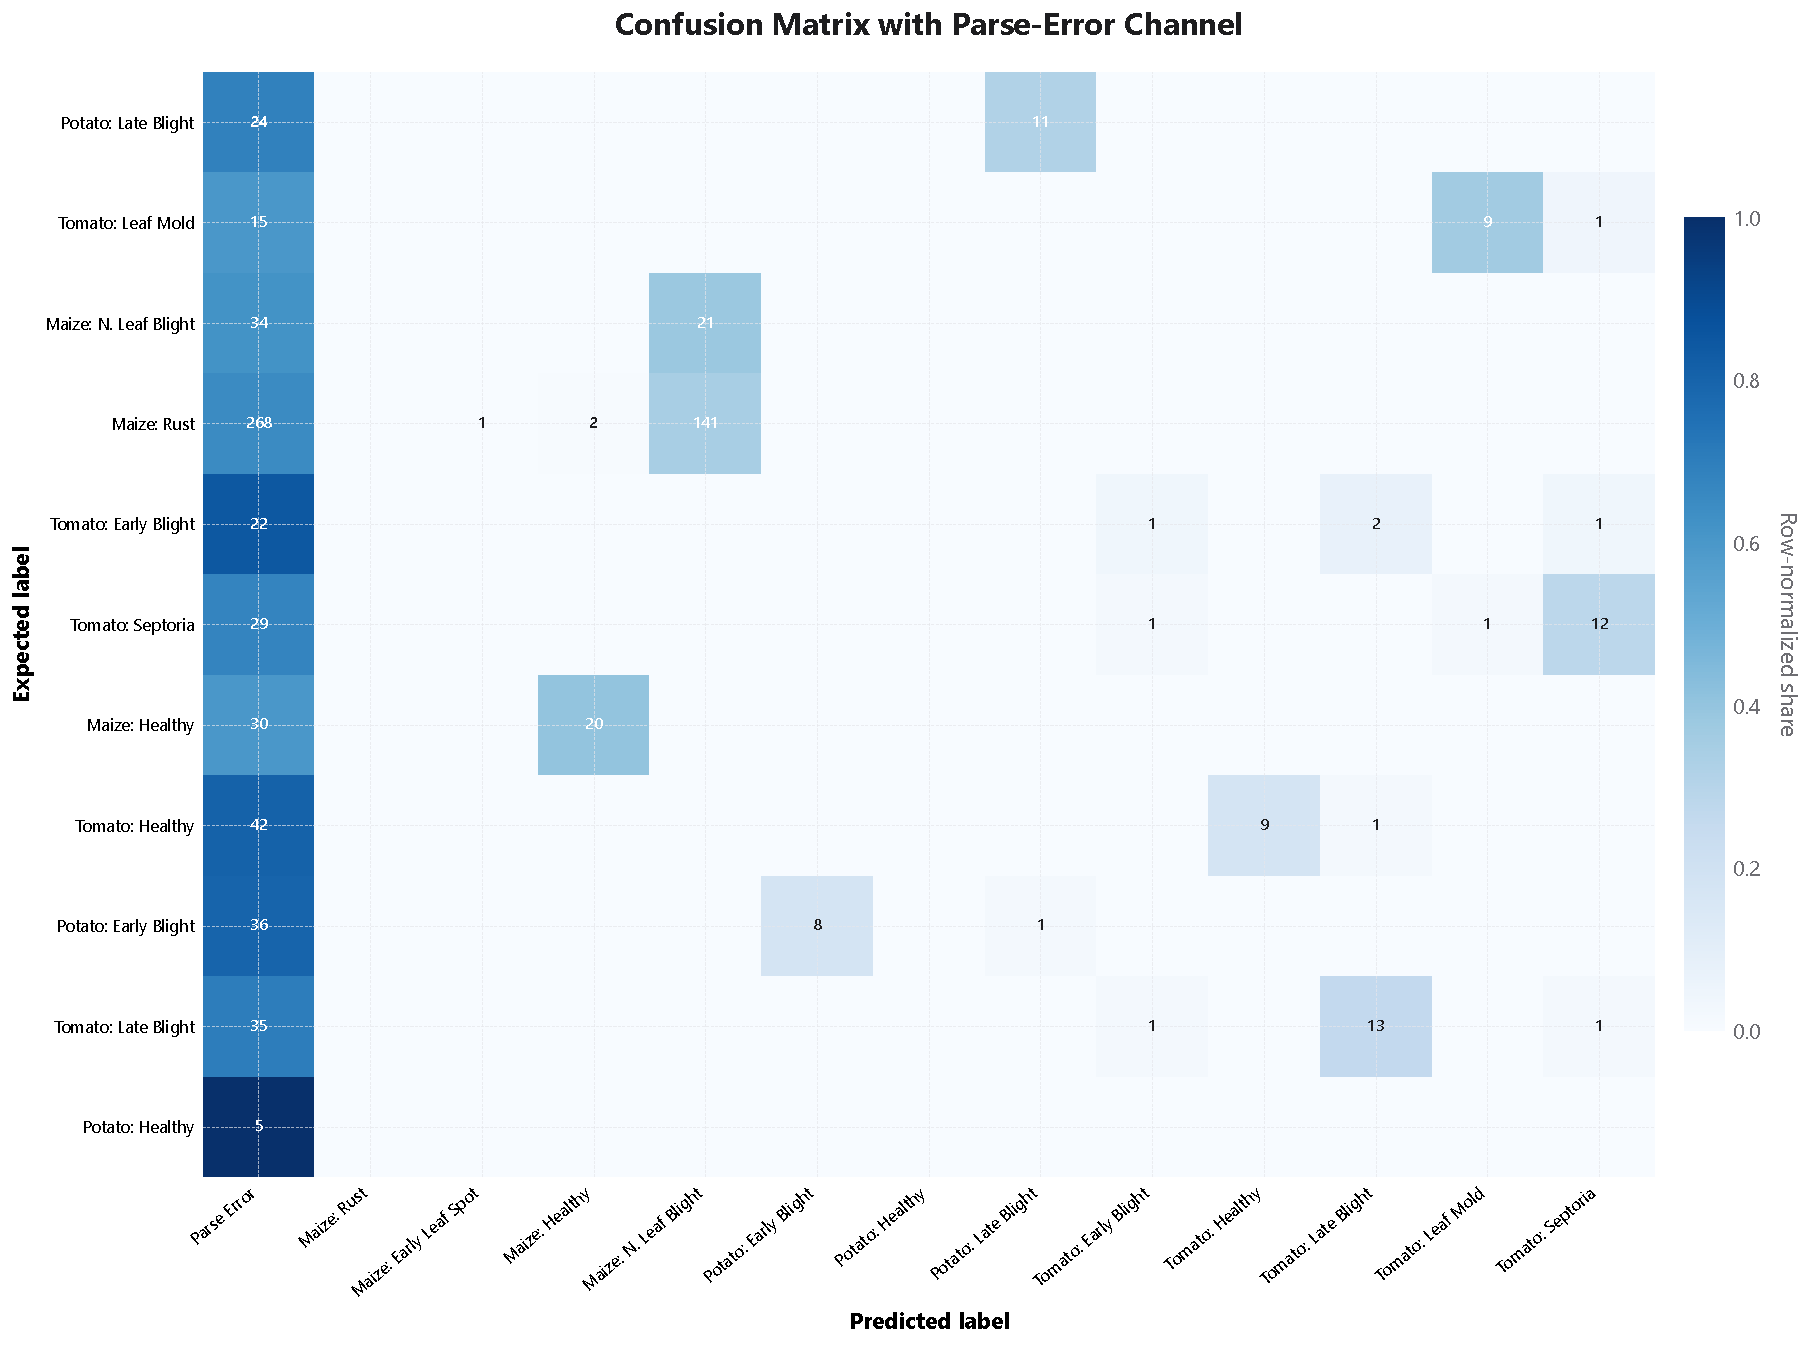
\includegraphics[height=0.4\textheight,keepaspectratio,width=0.95\textwidth]{data/krishi_vaidya_vlm_data/outputs/figures/figure5_confusion_matrix.pdf}
\caption{Confusion matrix for VLM prediction results}
\label{fig:vlm-confusion-matrix}
\end{figure}

\begin{figure}[H]
\centering
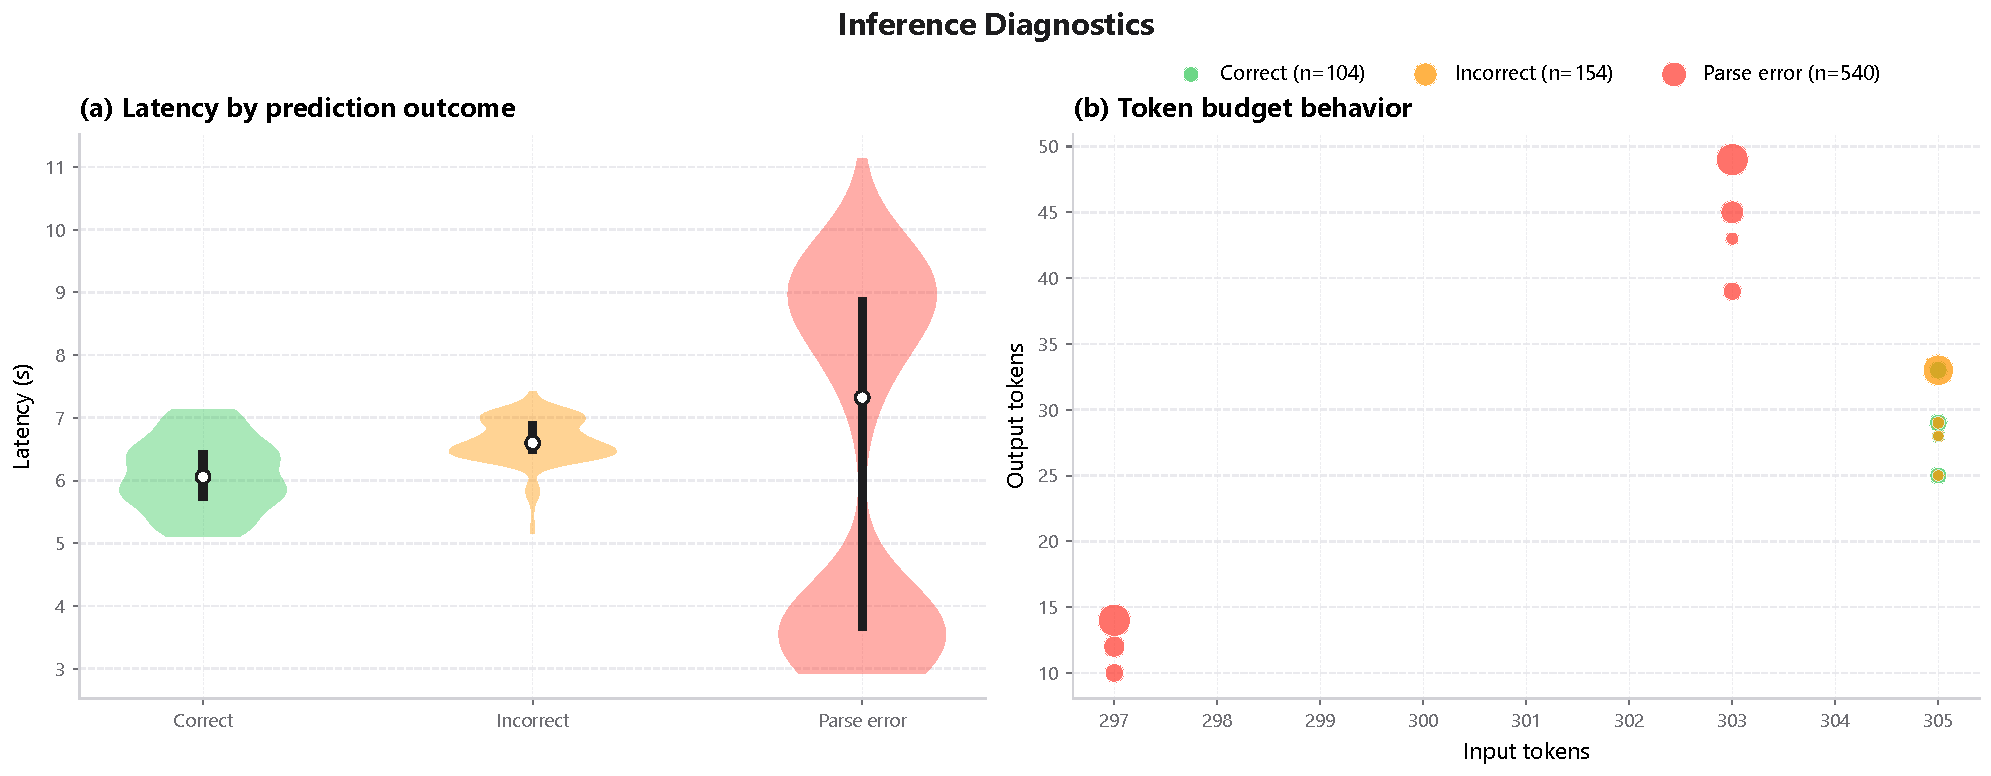
\includegraphics[height=0.45\textheight,keepaspectratio,width=\textwidth]{data/krishi_vaidya_vlm_data/outputs/figures/figure6_inference_diagnostics.pdf}
\caption{Inference diagnostics for VLM predictions}
\label{fig:vlm-inference-diagnostics}
\end{figure}

\subsubsection{Summary of VLM Findings}

The VLM work delivers a complete fine-tuning pipeline---dataset construction, LoRA adaptation,
quantized training, inference serving, and structured evaluation---within the NVIDIA L4 resource
envelope. Training converged successfully, but the prediction results show the model should not
yet serve as an autonomous disease classifier. The next improvement requires longer training,
better-balanced data, stricter output control, and possibly constrained decoding or
post-processing.

\ChapterSubsection{Backend Implementation Results}

The backend follows the layered architecture described in Chapter~4, implementing eight API
domains across configuration, middleware, routes, controllers, services, repositories, and
models. This section reports testing evidence and current limitations.

\subsubsection{Automated Test Coverage}

Automated tests focus on the scan domain. Twenty-one scan-service unit tests cover creation,
ownership, filtering, updating, soft deletion, statistics, resolution, and grouping.
Twenty-six scan-route integration tests cover authentication, pagination, validation, status
retrieval, resolution, and related-scan lookup. Both suites run against MongoDB Memory Server
with isolated test environments. Automated coverage was prioritized for local, repeatable
paths; the external VLM inference and Google AI integration within the diagnosis flow were
verified manually to control metered API costs. Remaining route groups---authentication,
crops, tasks, notes, and advisories---also rely on manual verification.

\subsubsection{Current Limitations}

Two design limitations remain. First, while Redis is initialized with BullMQ-compatible options,
diagnosis processing is currently synchronous; a scalable background-job pipeline remains future
work. Second, system reliability depends on upstream VLM and Google AI service availability, and
automated mocks for these external services have not yet been developed. These limitations do not
invalidate the backend as a complete API layer, but they define the boundary of its current
automated verification.

\ChapterSubsection{Mobile App Implementation Results}

The mobile application implements the architecture described in Chapter~4. Physical-device
testing on Android confirms the complete farmer-facing workflow.
Figures~\ref{fig:mobile-onboarding-screens}--\ref{fig:mobile-crop-registration} present
representative screenshots from on-device builds.

\begin{figure}[H]
\centering
\begin{minipage}[t]{0.49\textwidth}
\centering
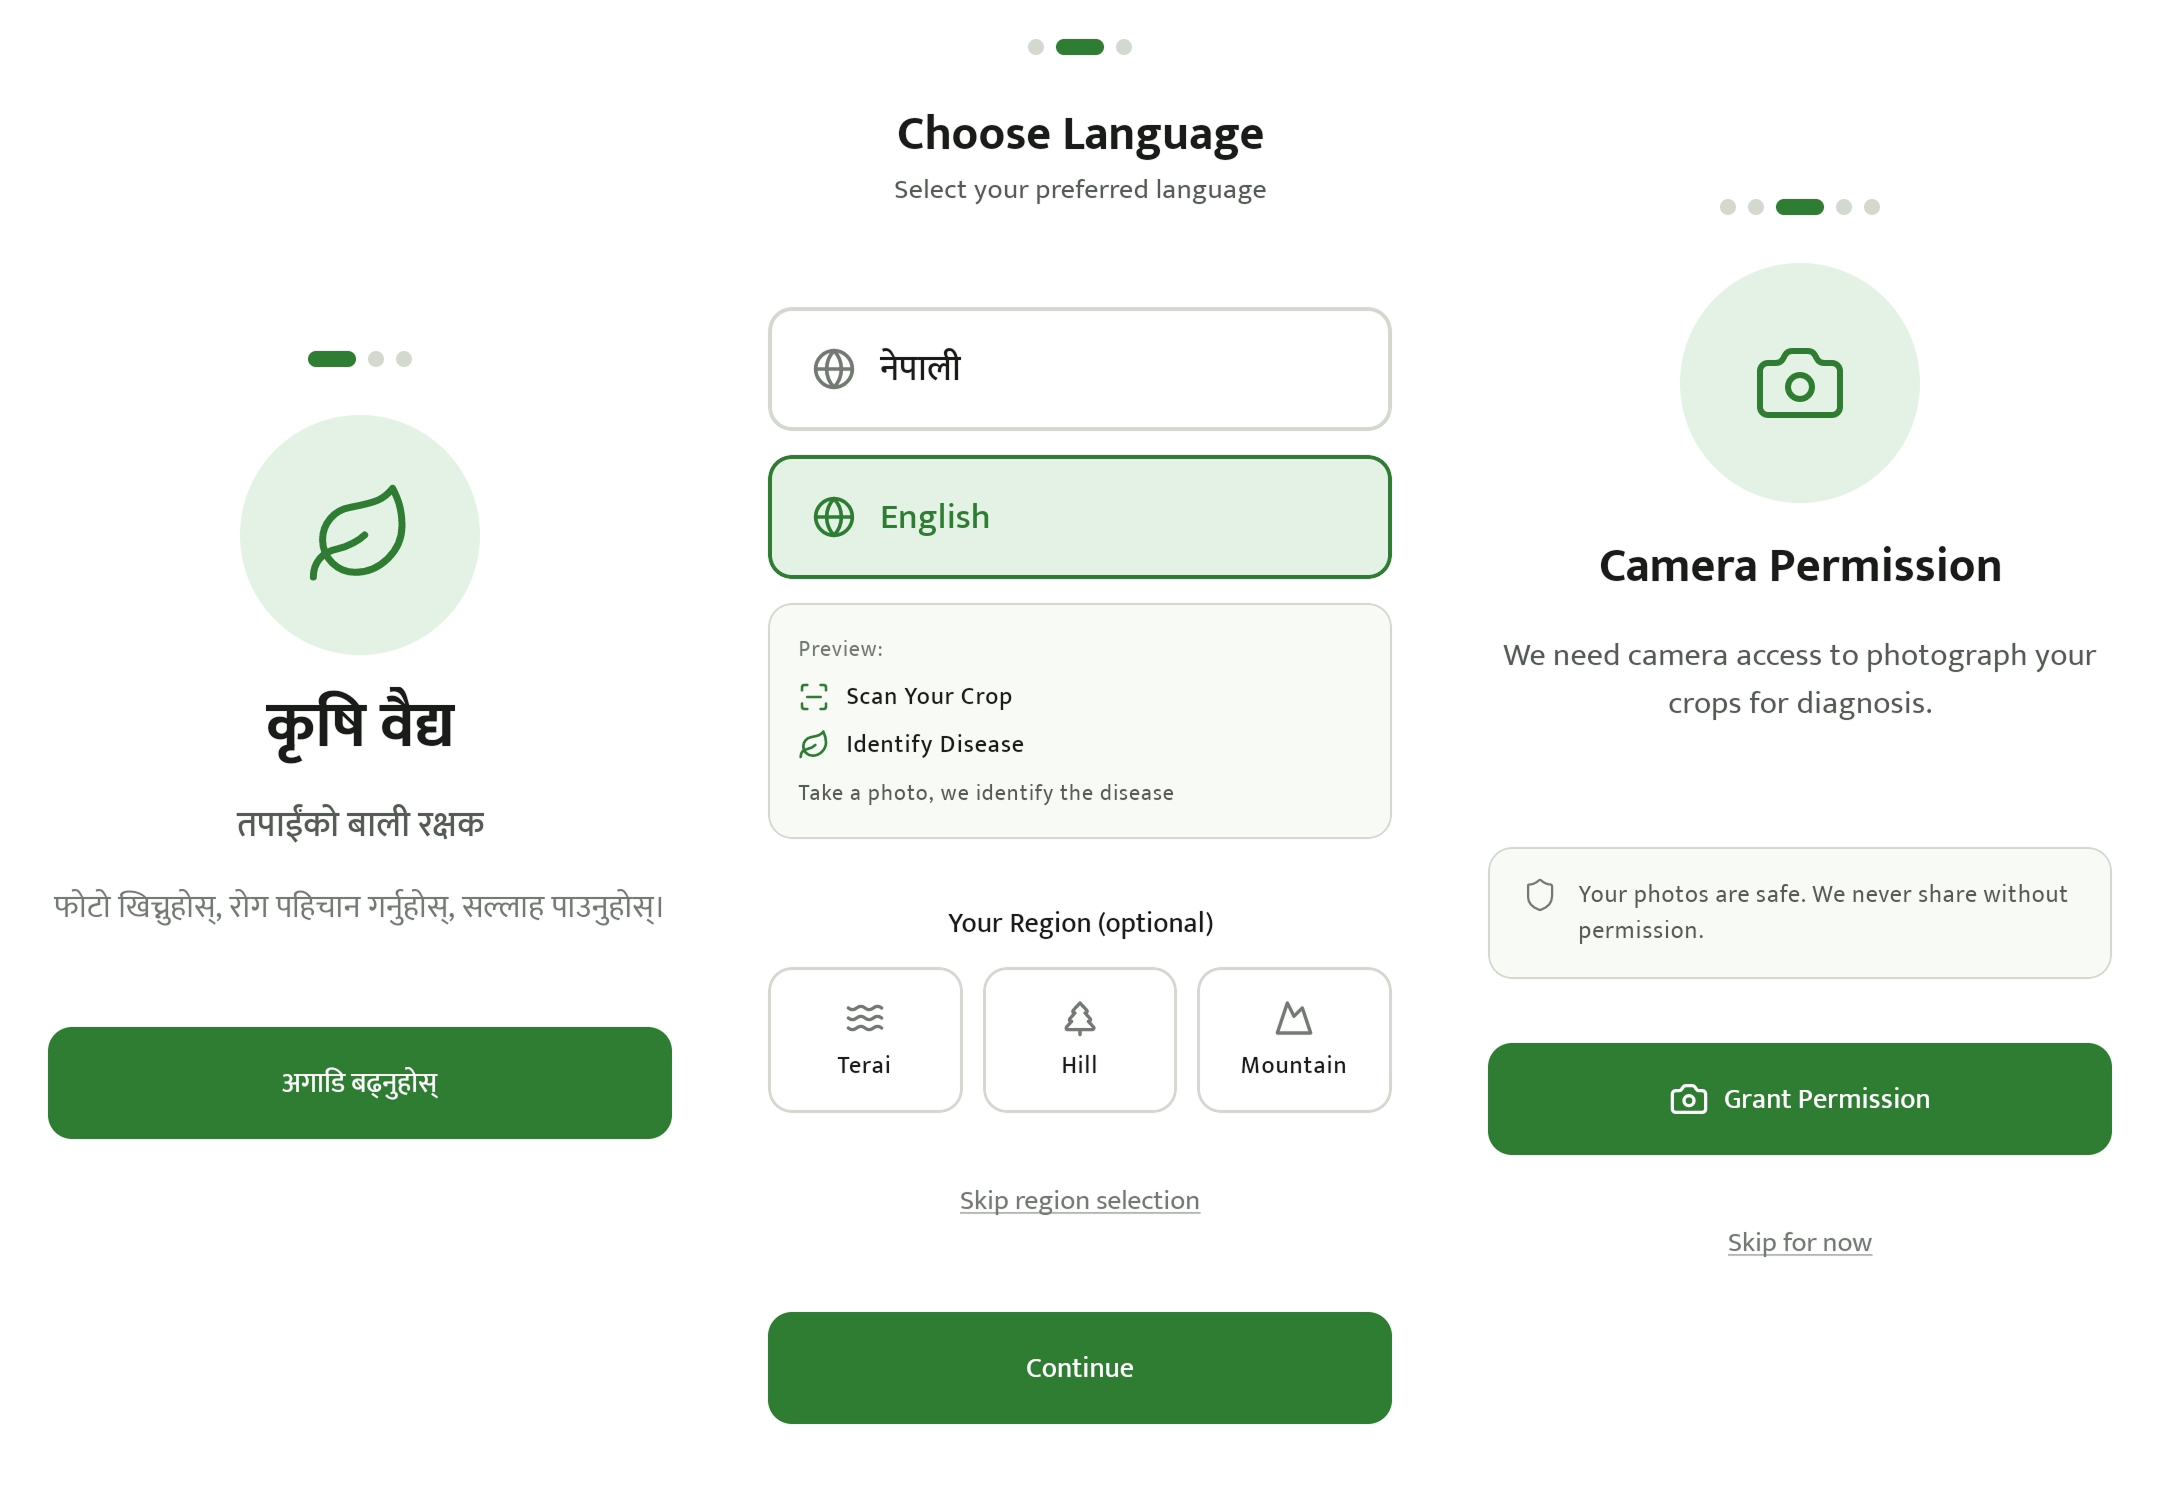
\includegraphics[height=0.3\textheight,keepaspectratio,width=\linewidth]{data/krishi_vaidya_mobile_app_data/onboarding/onboarding_2.png}
\end{minipage}\hfill
\begin{minipage}[t]{0.49\textwidth}
\centering
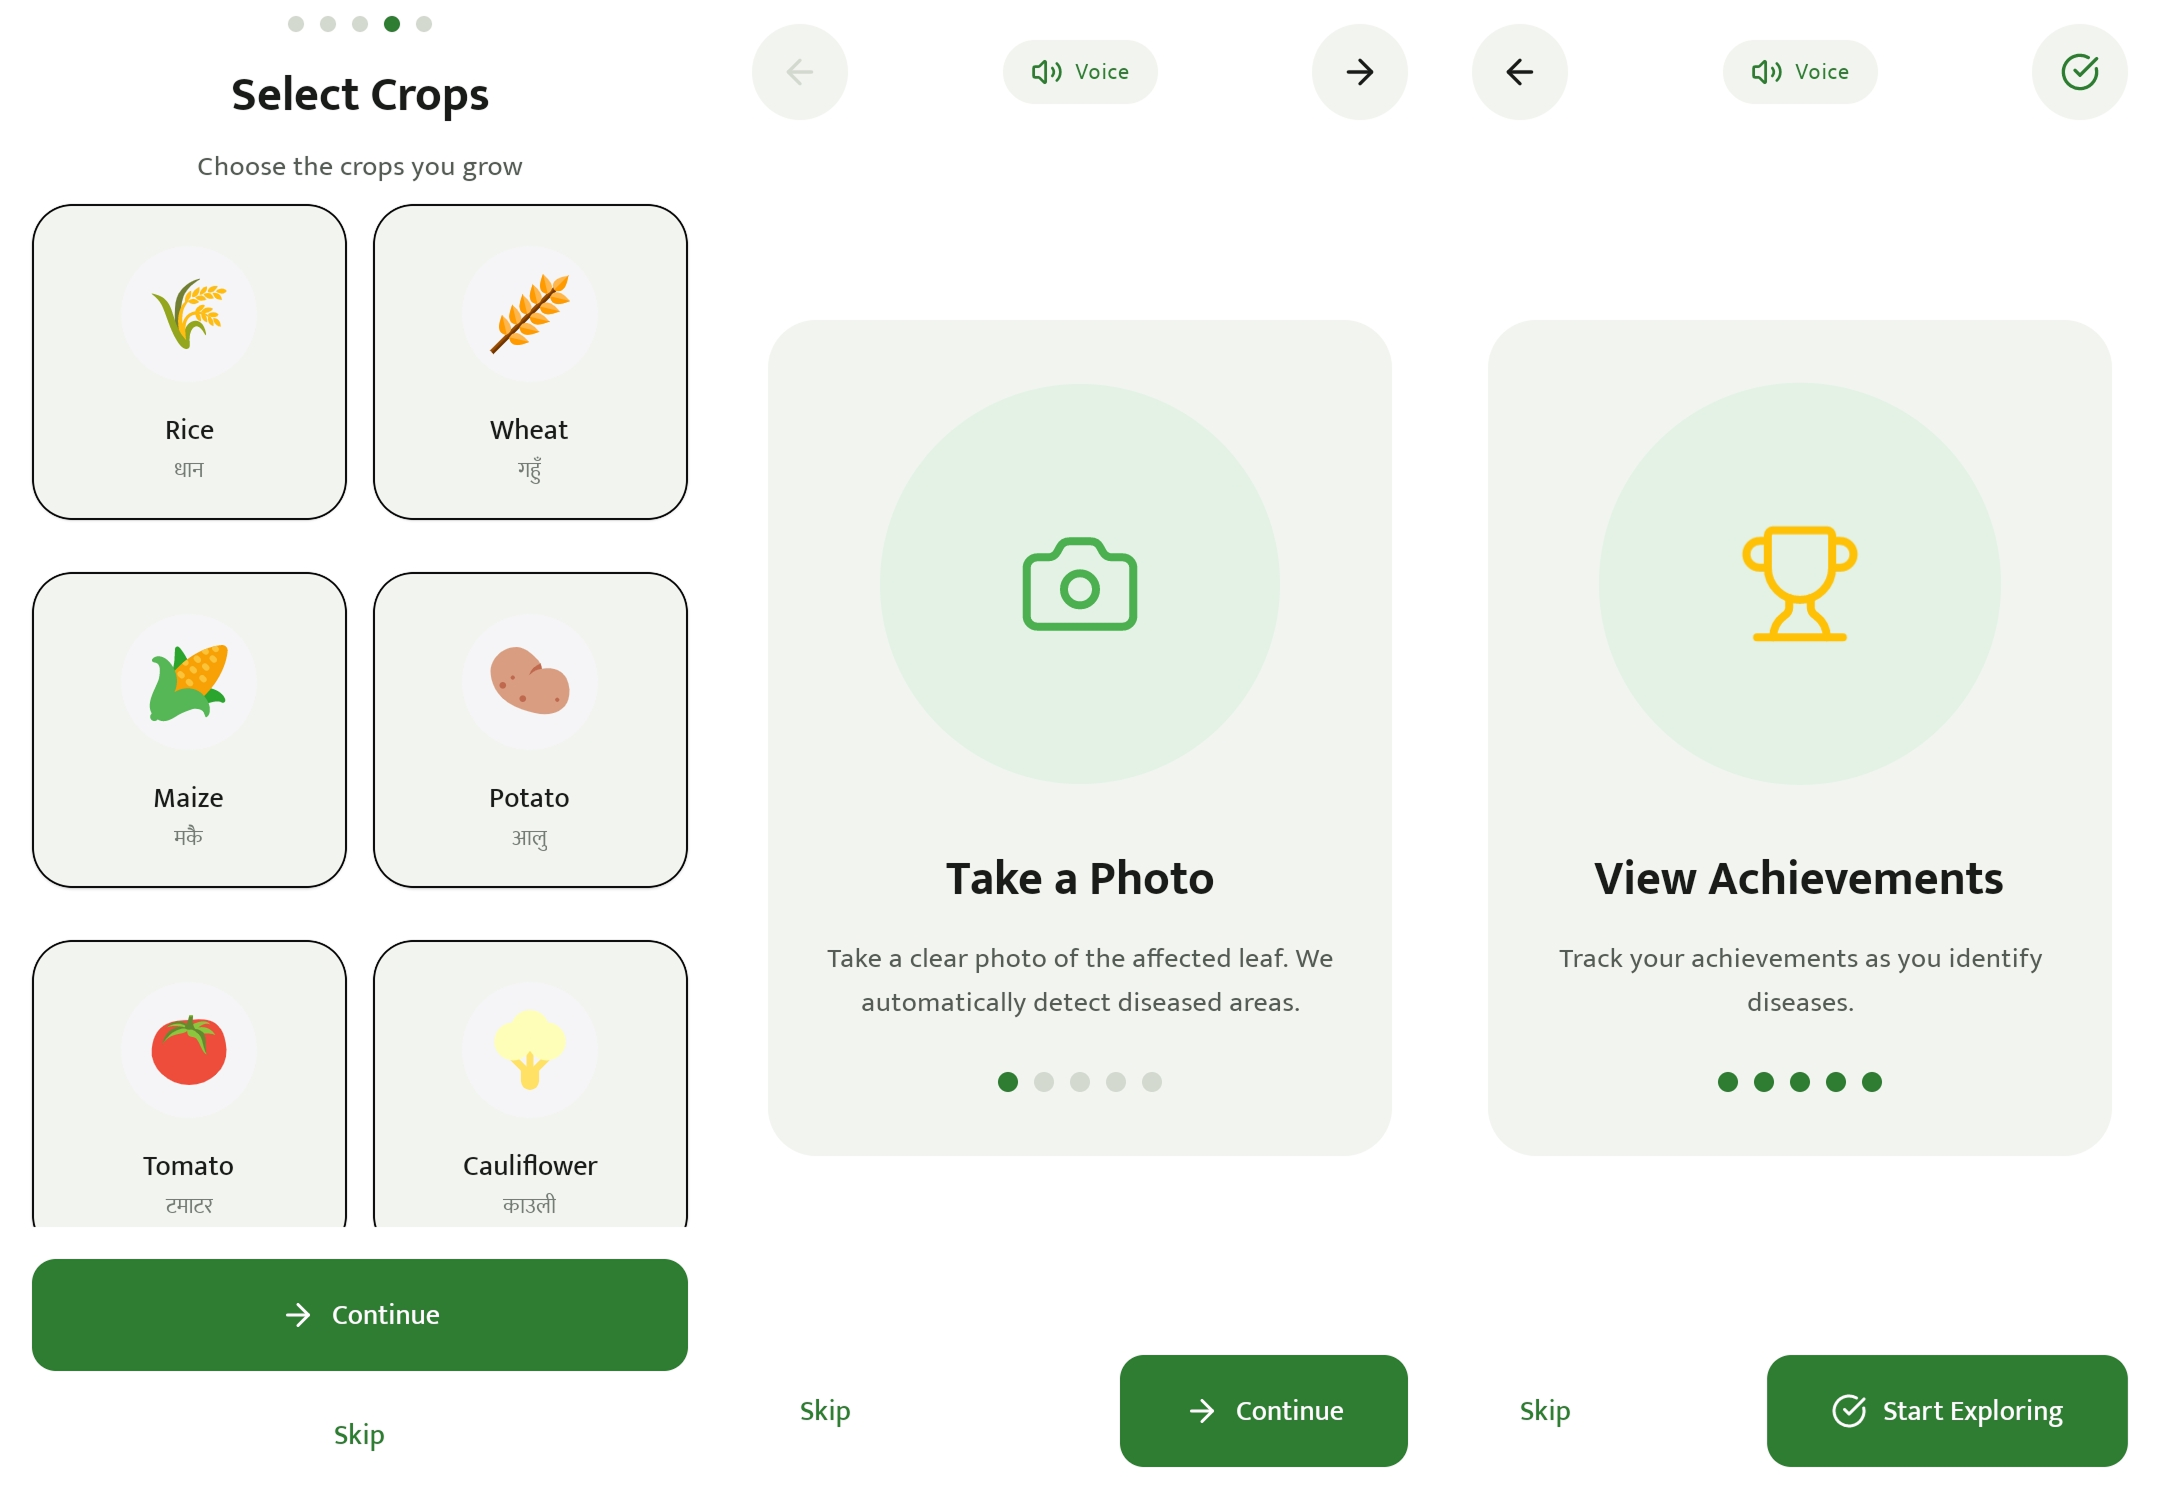
\includegraphics[height=0.3\textheight,keepaspectratio,width=\linewidth]{data/krishi_vaidya_mobile_app_data/onboarding/onboarding_1.png}
\end{minipage}
\caption{First-run onboarding screenshots showing language selection, camera permission, crop selection, and completion.}
\label{fig:mobile-onboarding-screens}
\end{figure}

\begin{figure}[H]
\centering
\begin{minipage}[t]{0.49\textwidth}
\centering
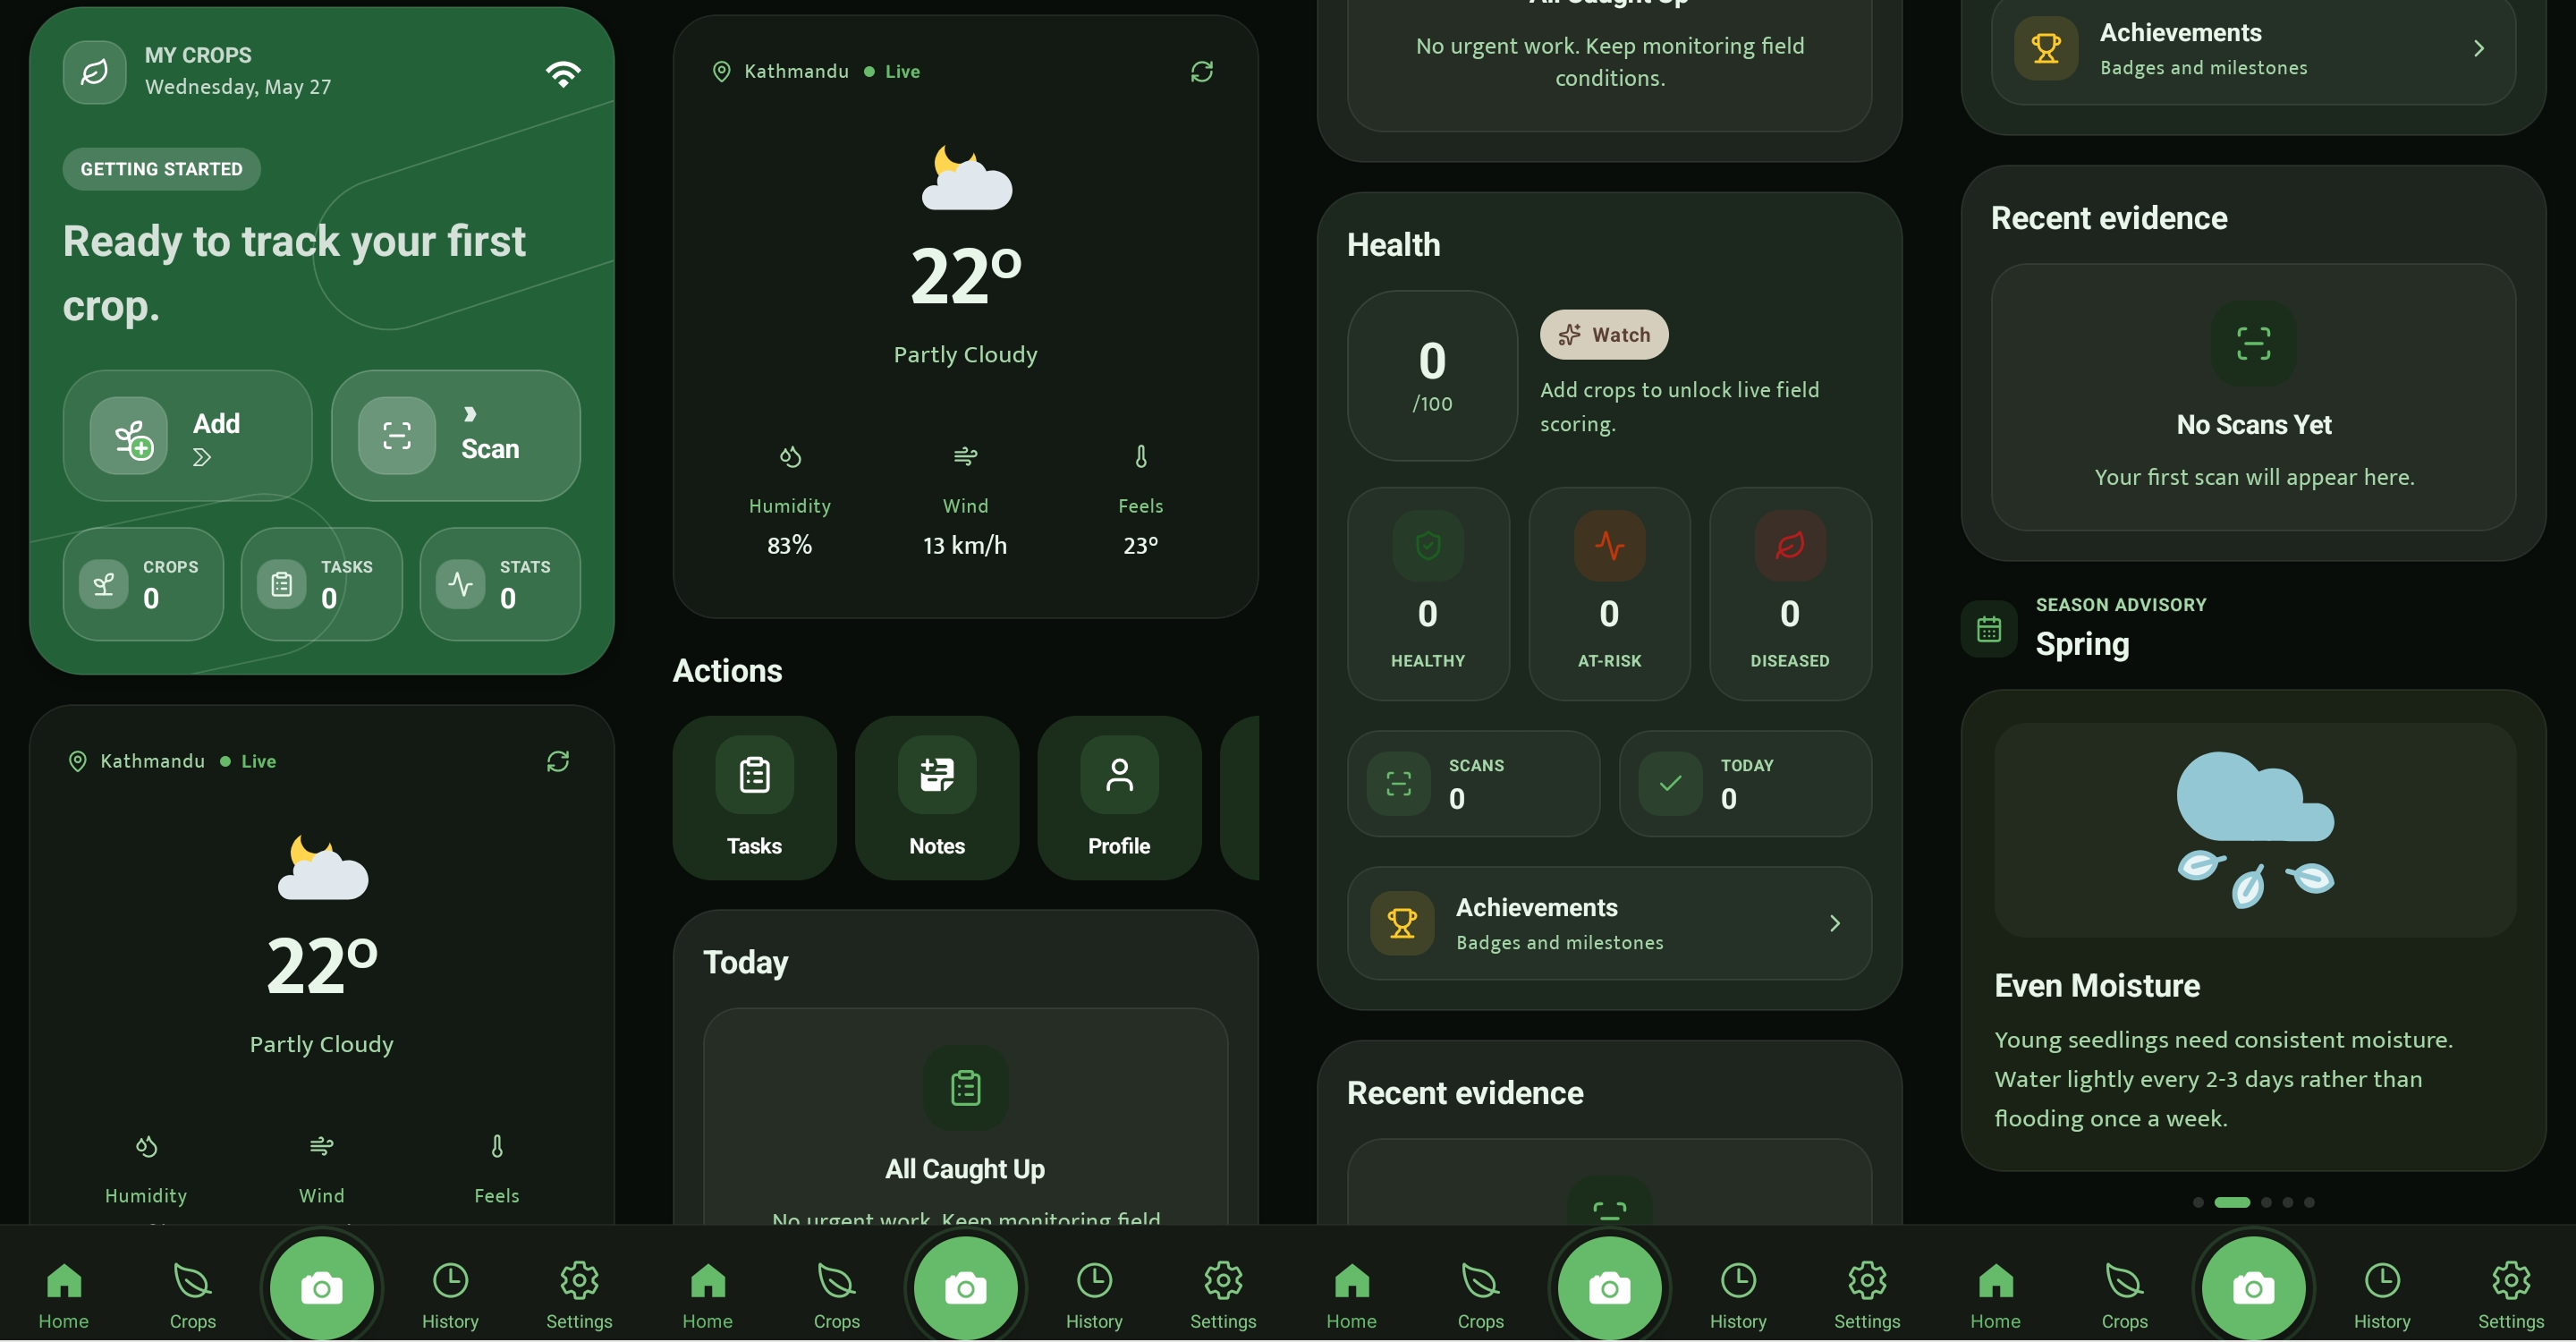
\includegraphics[height=0.3\textheight,keepaspectratio,width=\linewidth]{data/krishi_vaidya_mobile_app_data/homepage/home.png}
\end{minipage}\hfill
\begin{minipage}[t]{0.49\textwidth}
\centering
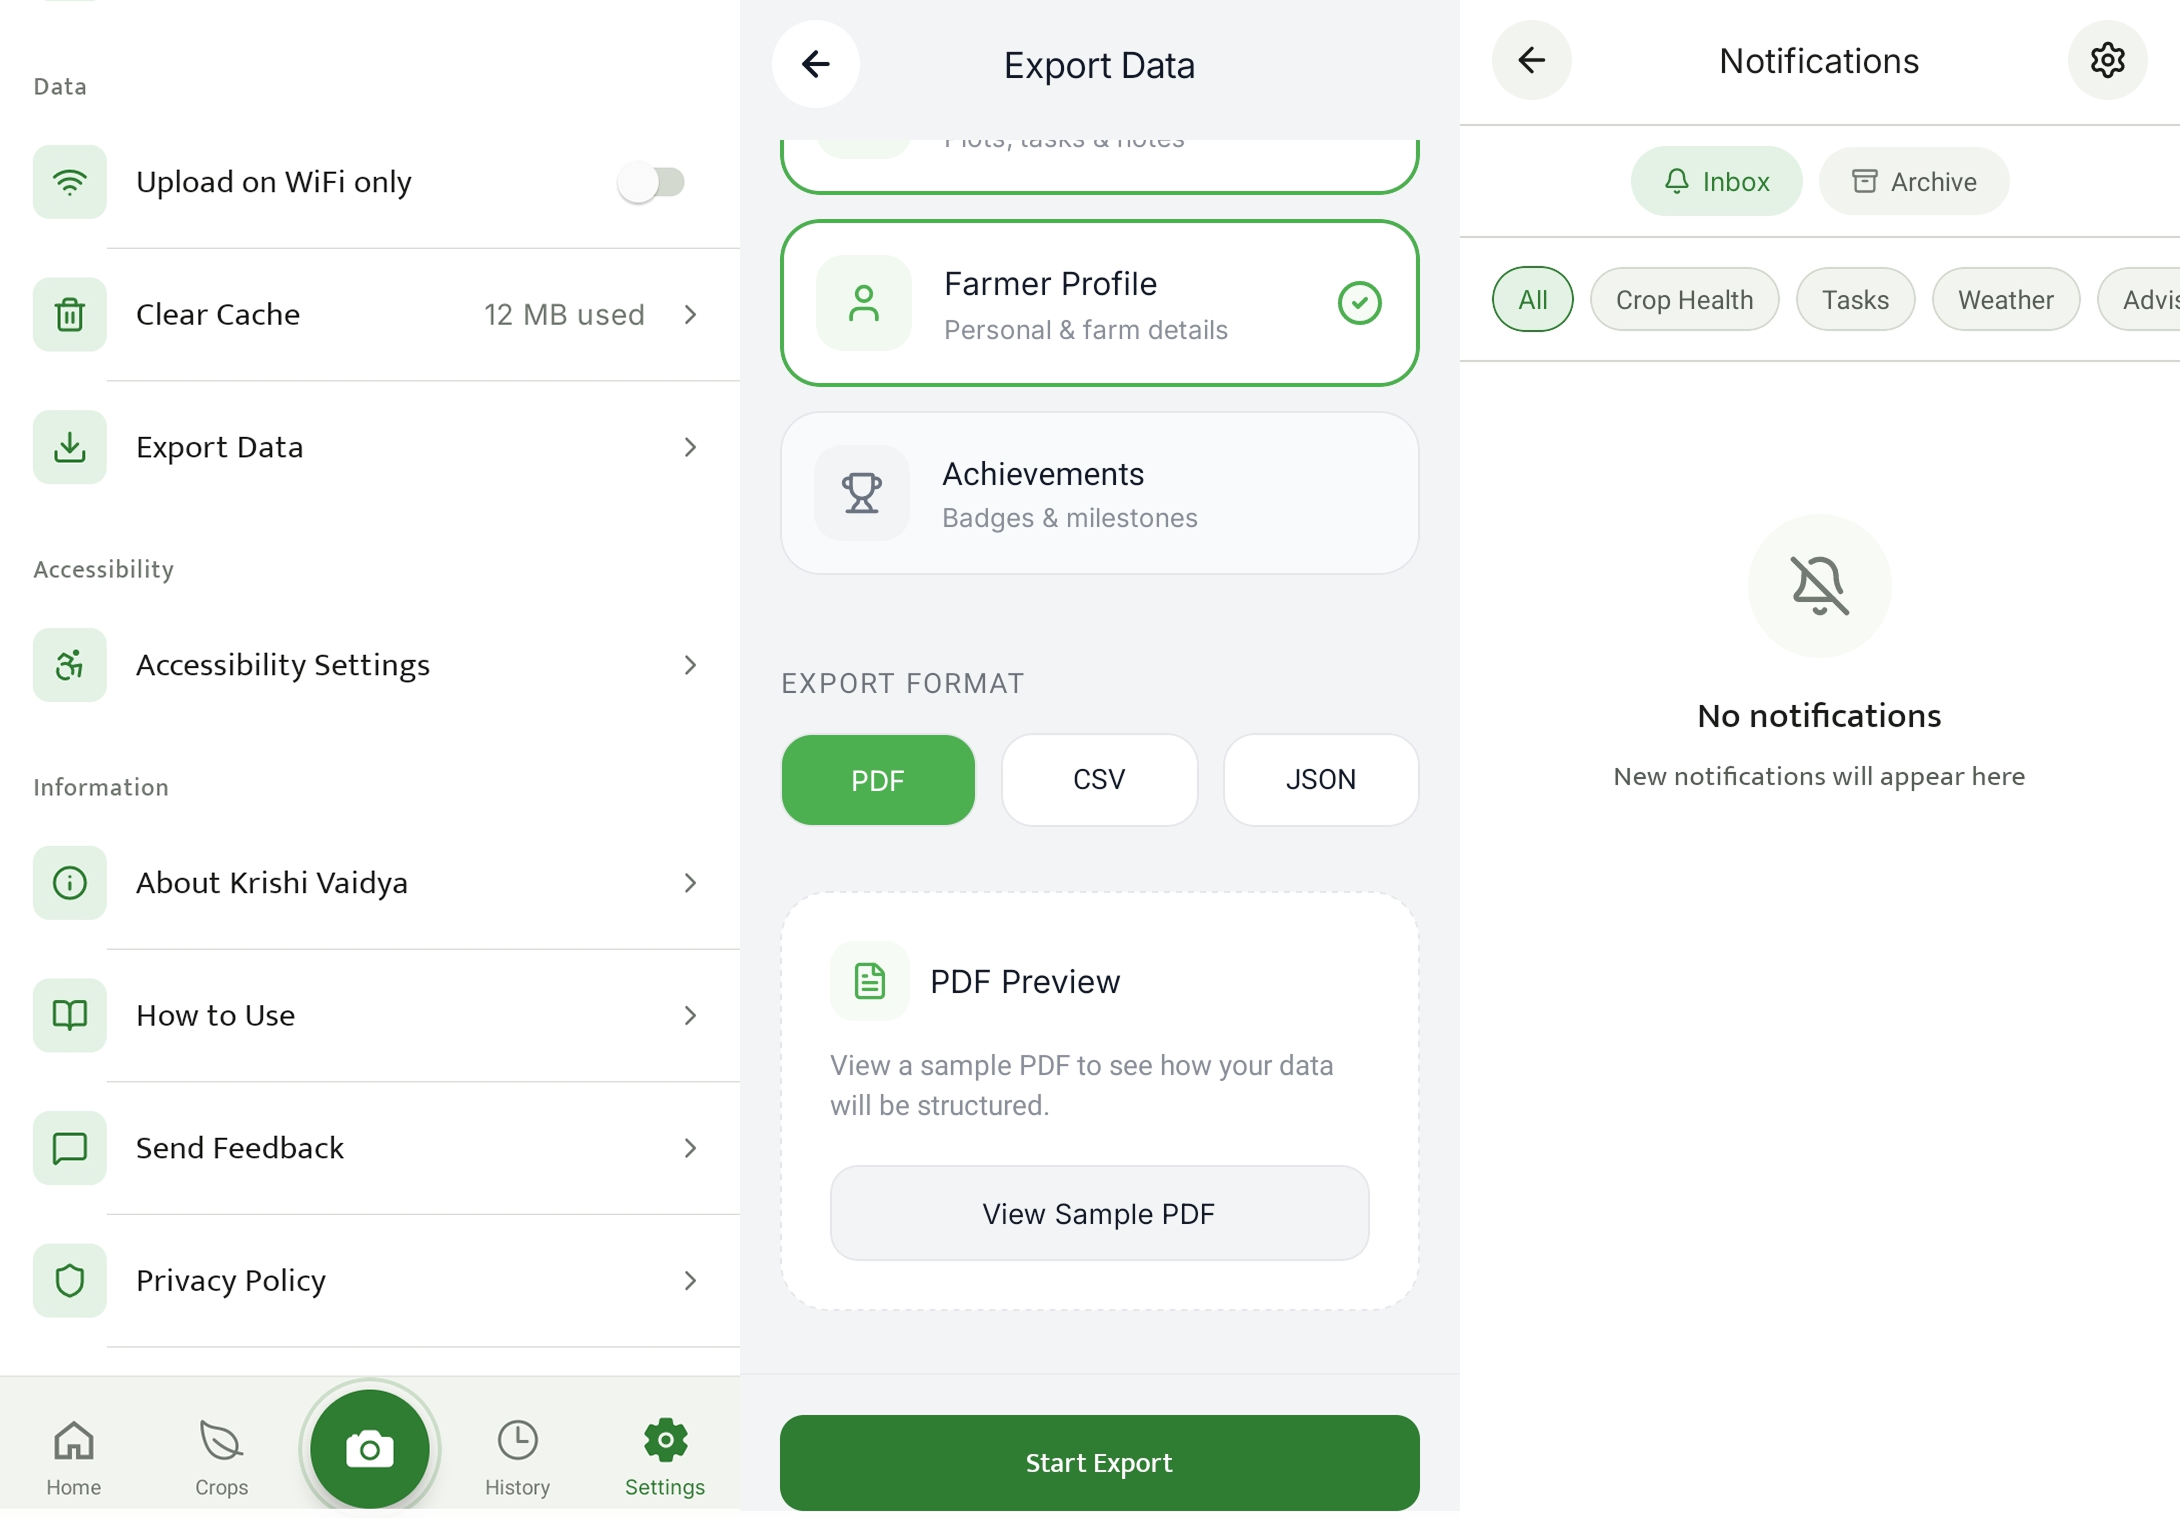
\includegraphics[height=0.3\textheight,keepaspectratio,width=\linewidth]{data/krishi_vaidya_mobile_app_data/settings/settings.png}
\end{minipage}
\caption{Dashboard and settings screenshots showing the home surface, crop summary, notifications, and accessibility configuration.}
\label{fig:mobile-home-settings-screens}
\end{figure}

\subsubsection{Scan and Diagnosis Workflow}

The scan workflow operates as a controlled multi-stage sequence: capture with crop context,
preview with quality analysis, optional image editing, detection, cloud diagnosis submission,
and structured report display. The cloud path submits multipart payloads to
\texttt{/api/v1/diagnose}, with network-aware behavior: online connections trigger cloud
execution, slow connections race against a five-second timeout, and offline states queue the
payload while checking for cached advisories. The result view renders disease etiology, treatment
timelines, organic alternatives, and text-to-speech output, with PDF export and reminder support.

\begin{figure}[H]
\centering
\begin{minipage}[t]{0.49\textwidth}
\centering
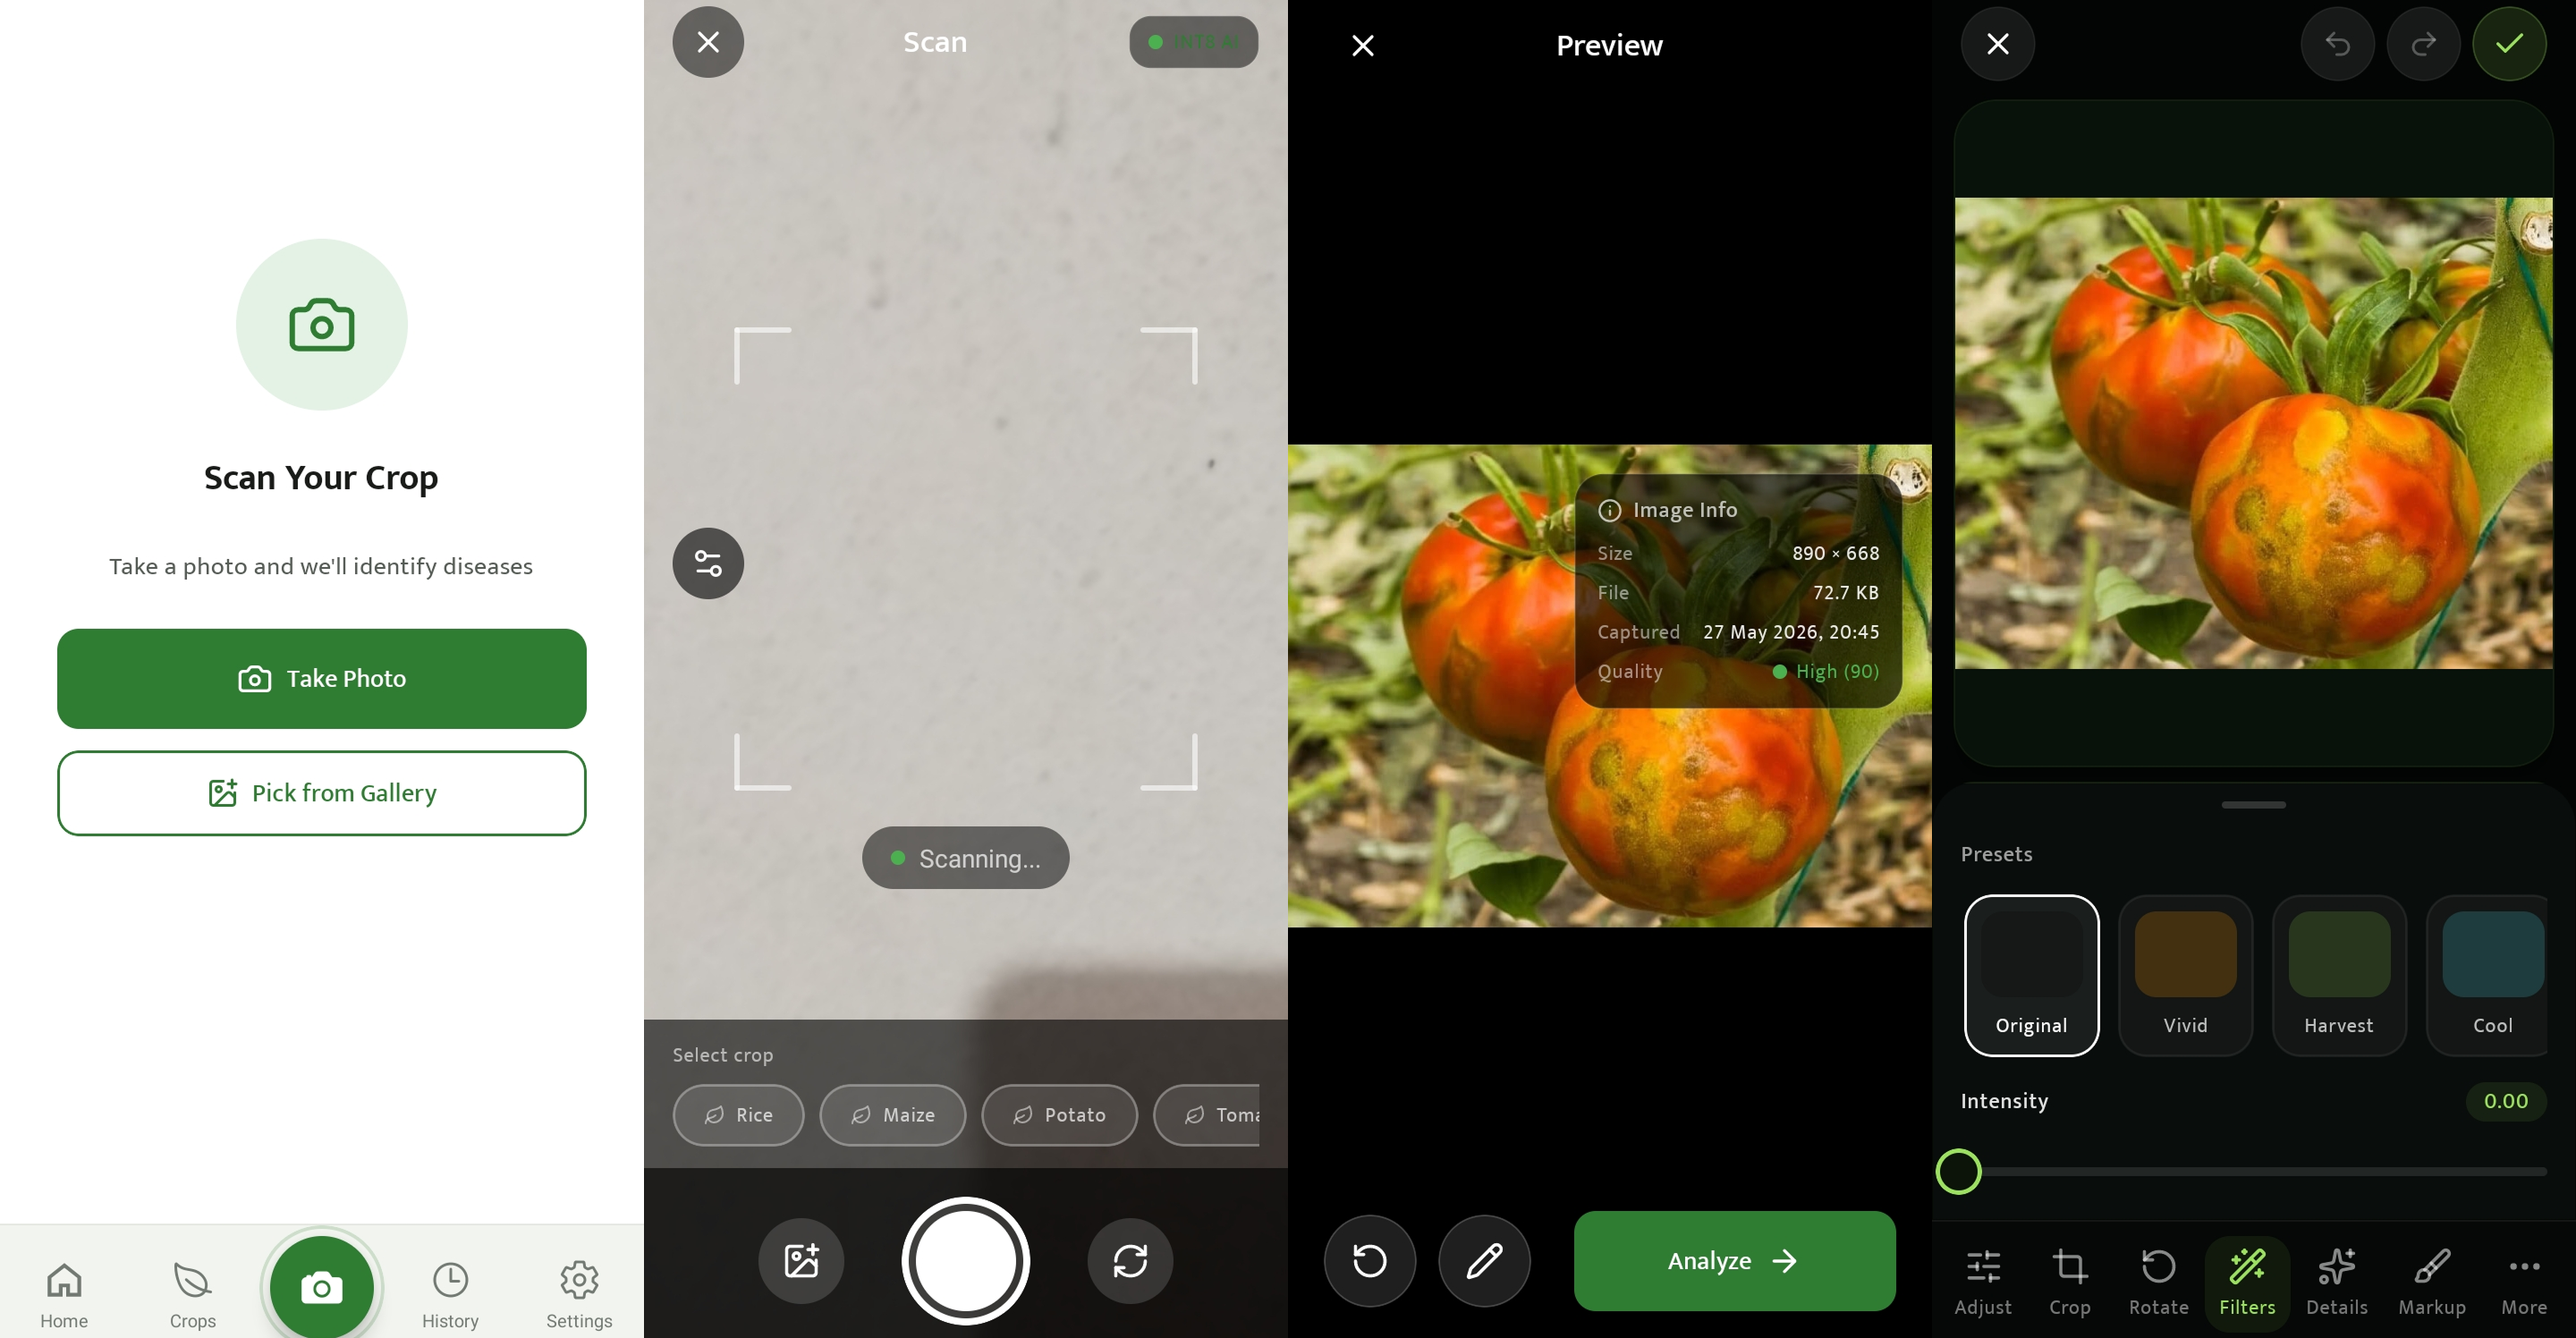
\includegraphics[height=0.3\textheight,keepaspectratio,width=\linewidth]{data/krishi_vaidya_mobile_app_data/scan/scan_1.png}
\end{minipage}\hfill
\begin{minipage}[t]{0.49\textwidth}
\centering
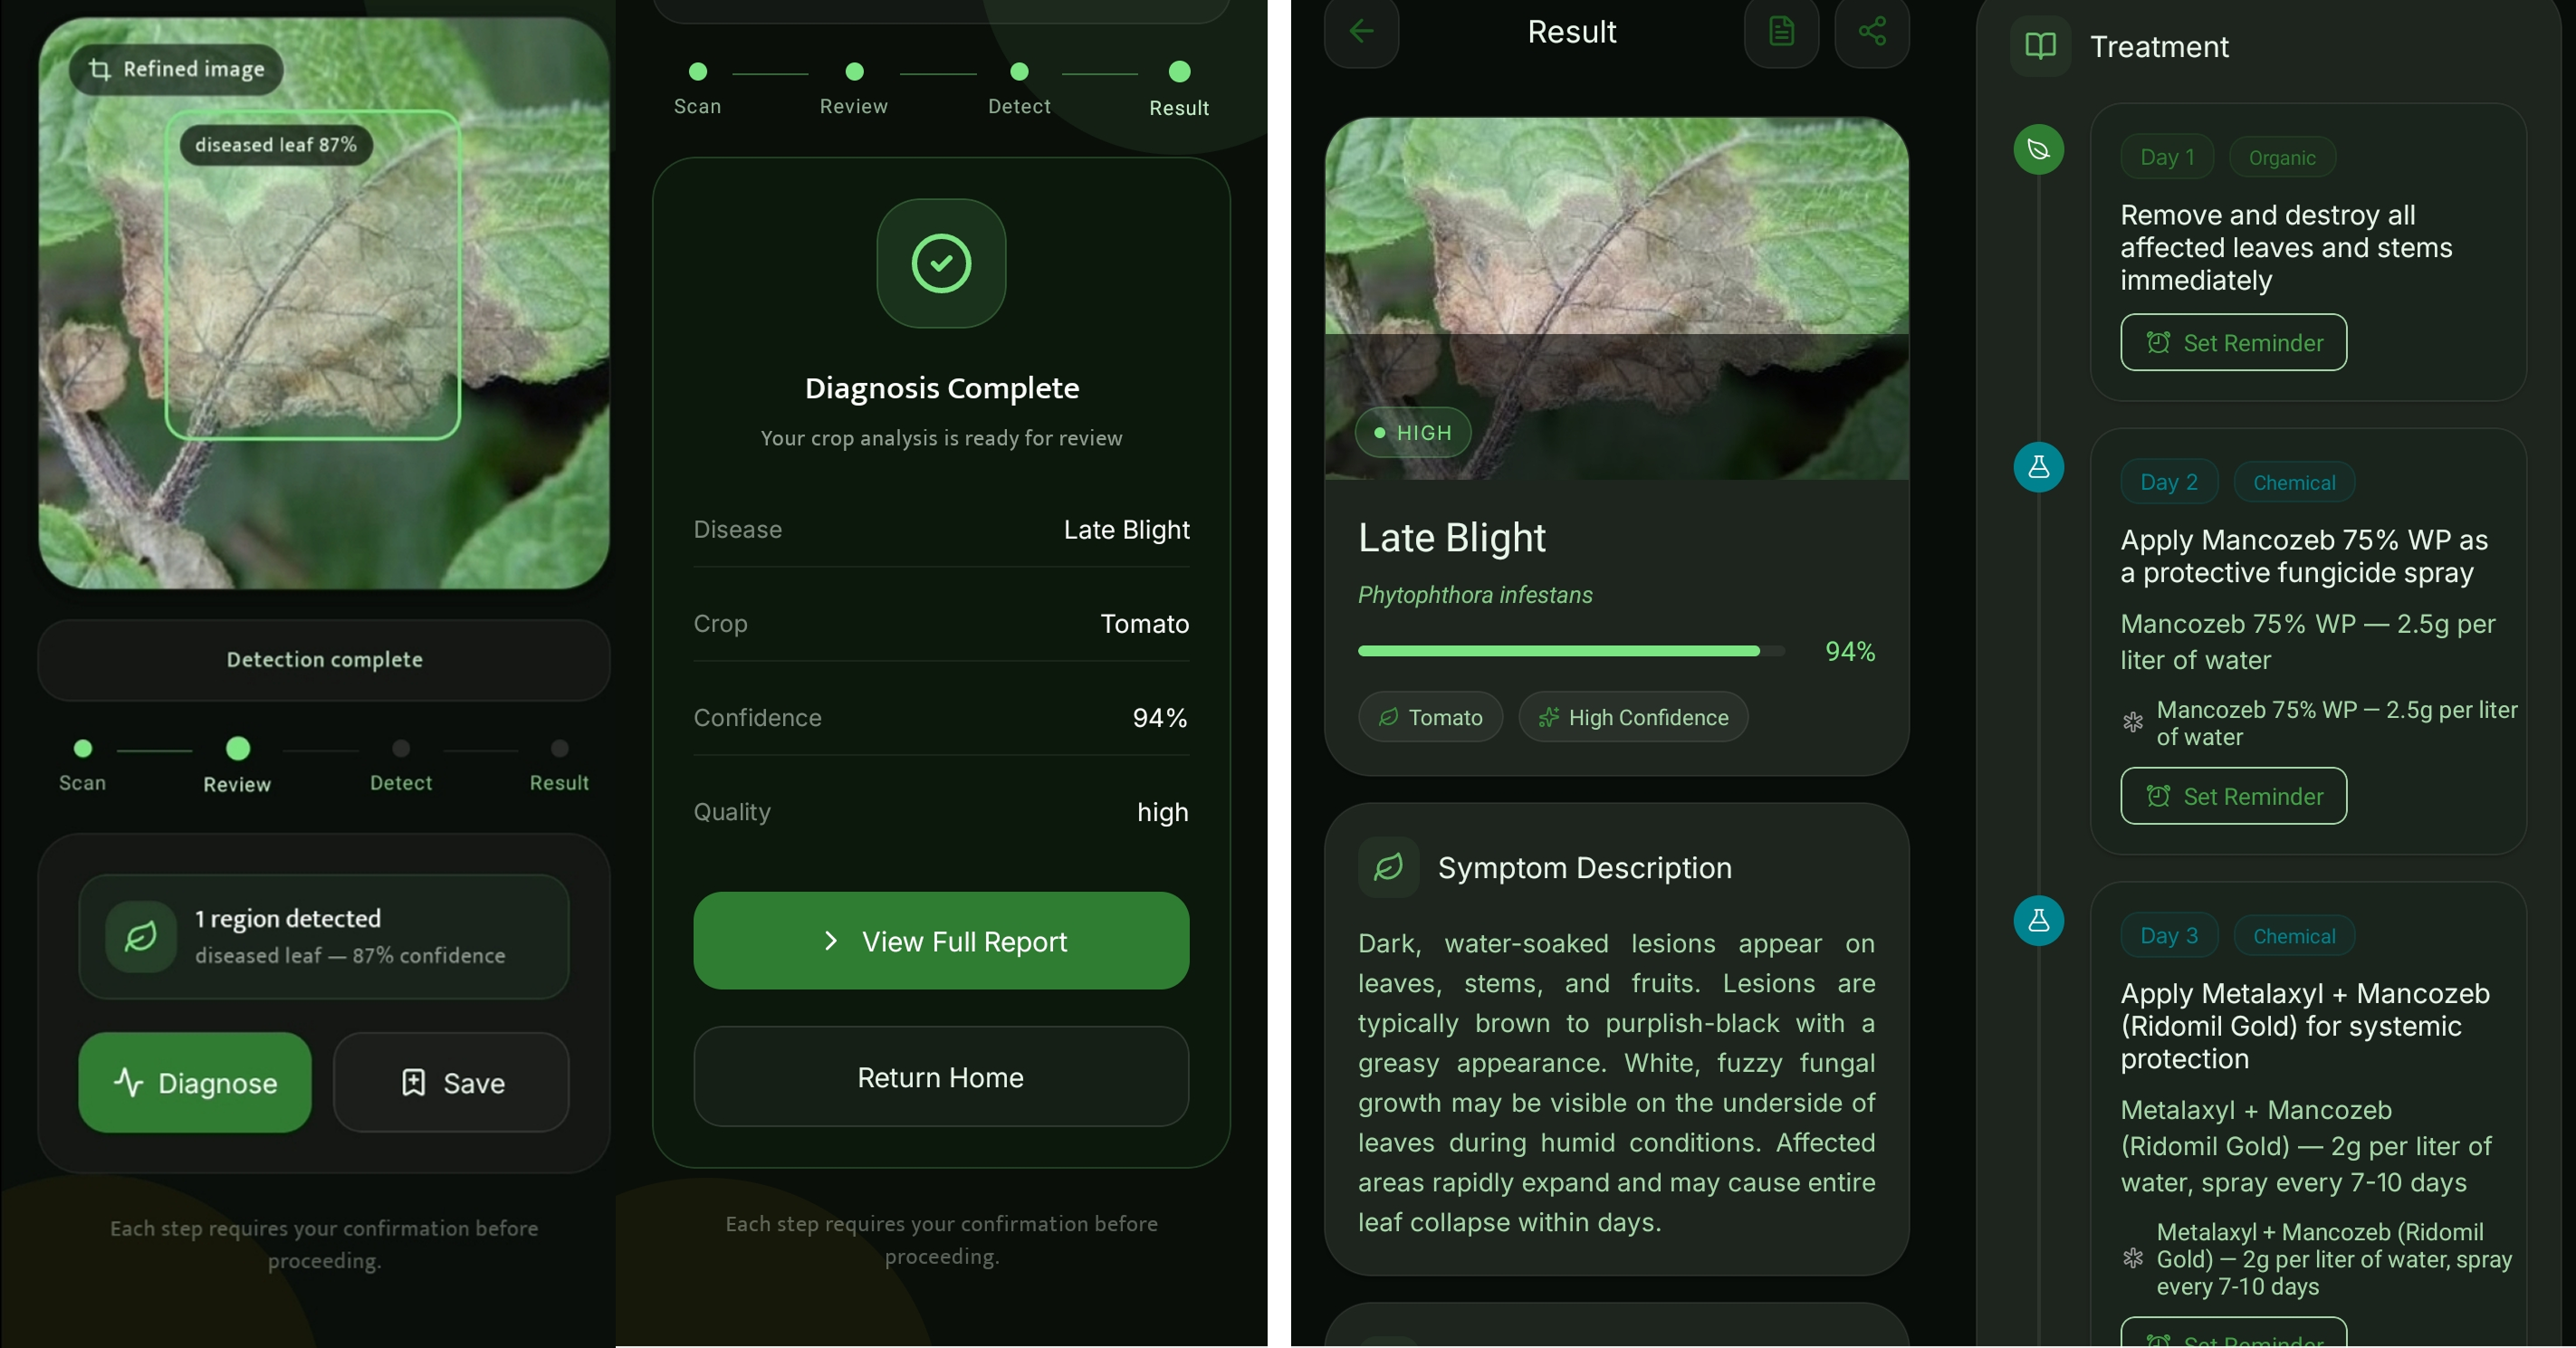
\includegraphics[height=0.3\textheight,keepaspectratio,width=\linewidth]{data/krishi_vaidya_mobile_app_data/scan/scan_2.png}
\end{minipage}
\caption{Scan and diagnosis screenshots showing capture, preview, diagnosis completion, structured result display, and treatment guidance.}
\label{fig:mobile-scan-workflow-screens}
\end{figure}

\subsubsection{Offline Support and Crop Management}
SQLite persists scan history, queued uploads, crop plots, tasks, notes, advisories, settings,
and notifications.
\begin{figure}[H]
\centering
\begin{minipage}[t]{0.49\textwidth}
\centering
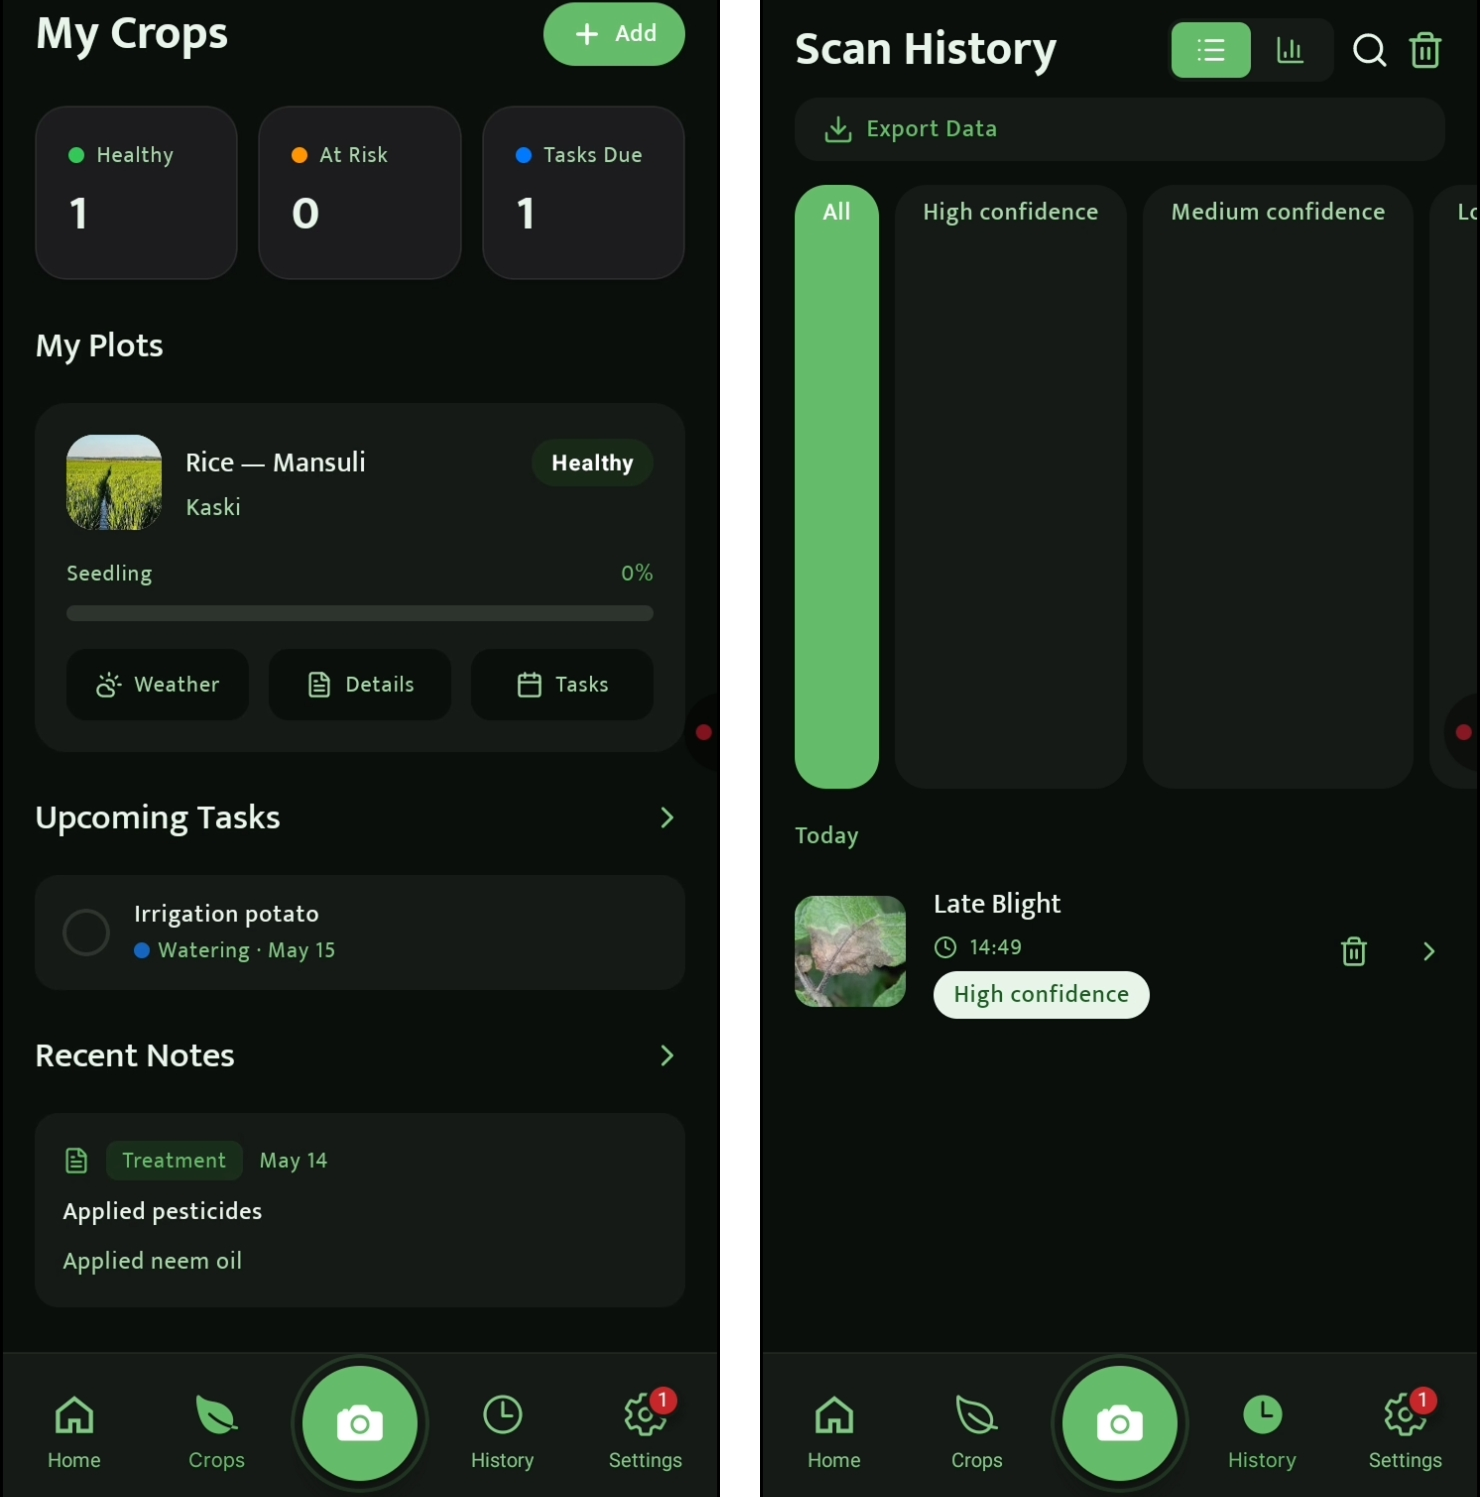
\includegraphics[height=0.3\textheight,keepaspectratio,width=\linewidth]{data/krishi_vaidya_mobile_app_data/crop/crops.png}
\end{minipage}\hfill
\begin{minipage}[t]{0.49\textwidth}
\centering
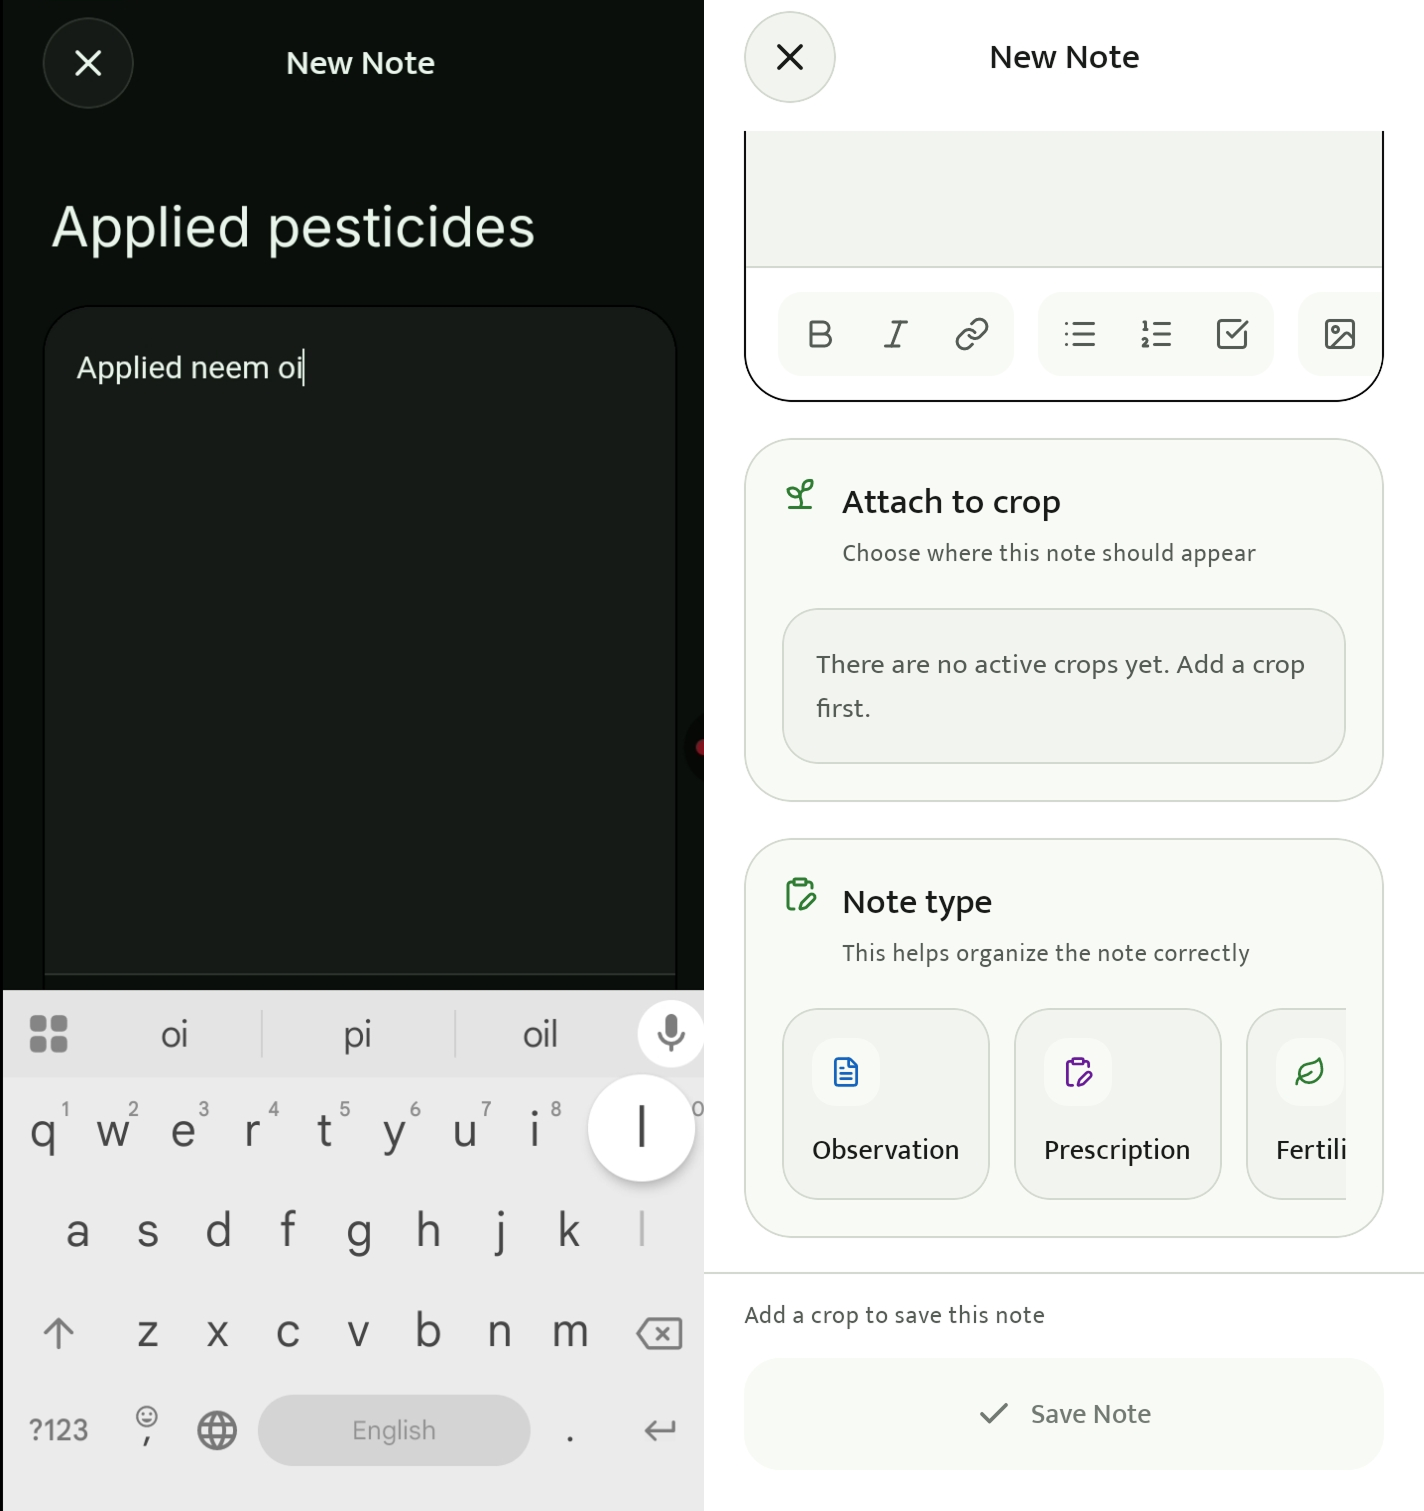
\includegraphics[height=0.3\textheight,keepaspectratio,width=\linewidth]{data/krishi_vaidya_mobile_app_data/notes/notes.png}
\end{minipage}
\caption{Crop management screenshots showing the crop dashboard and note creation.}
\label{fig:mobile-crop-management-screens}
\end{figure}
The sync manager monitors connectivity and processes queued operations in
batches. Core offline-to-online queue recovery is verified, though full bidirectional
synchronization for secondary tables awaits matching backend handlers.

The crop dashboard aggregates active plots, upcoming tasks, recent notes, active advisories,
and weather context. Figures~\ref{fig:mobile-crop-management-screens}
and~\ref{fig:mobile-crop-registration} show the crop management interface.


\begin{figure}[H]
\centering
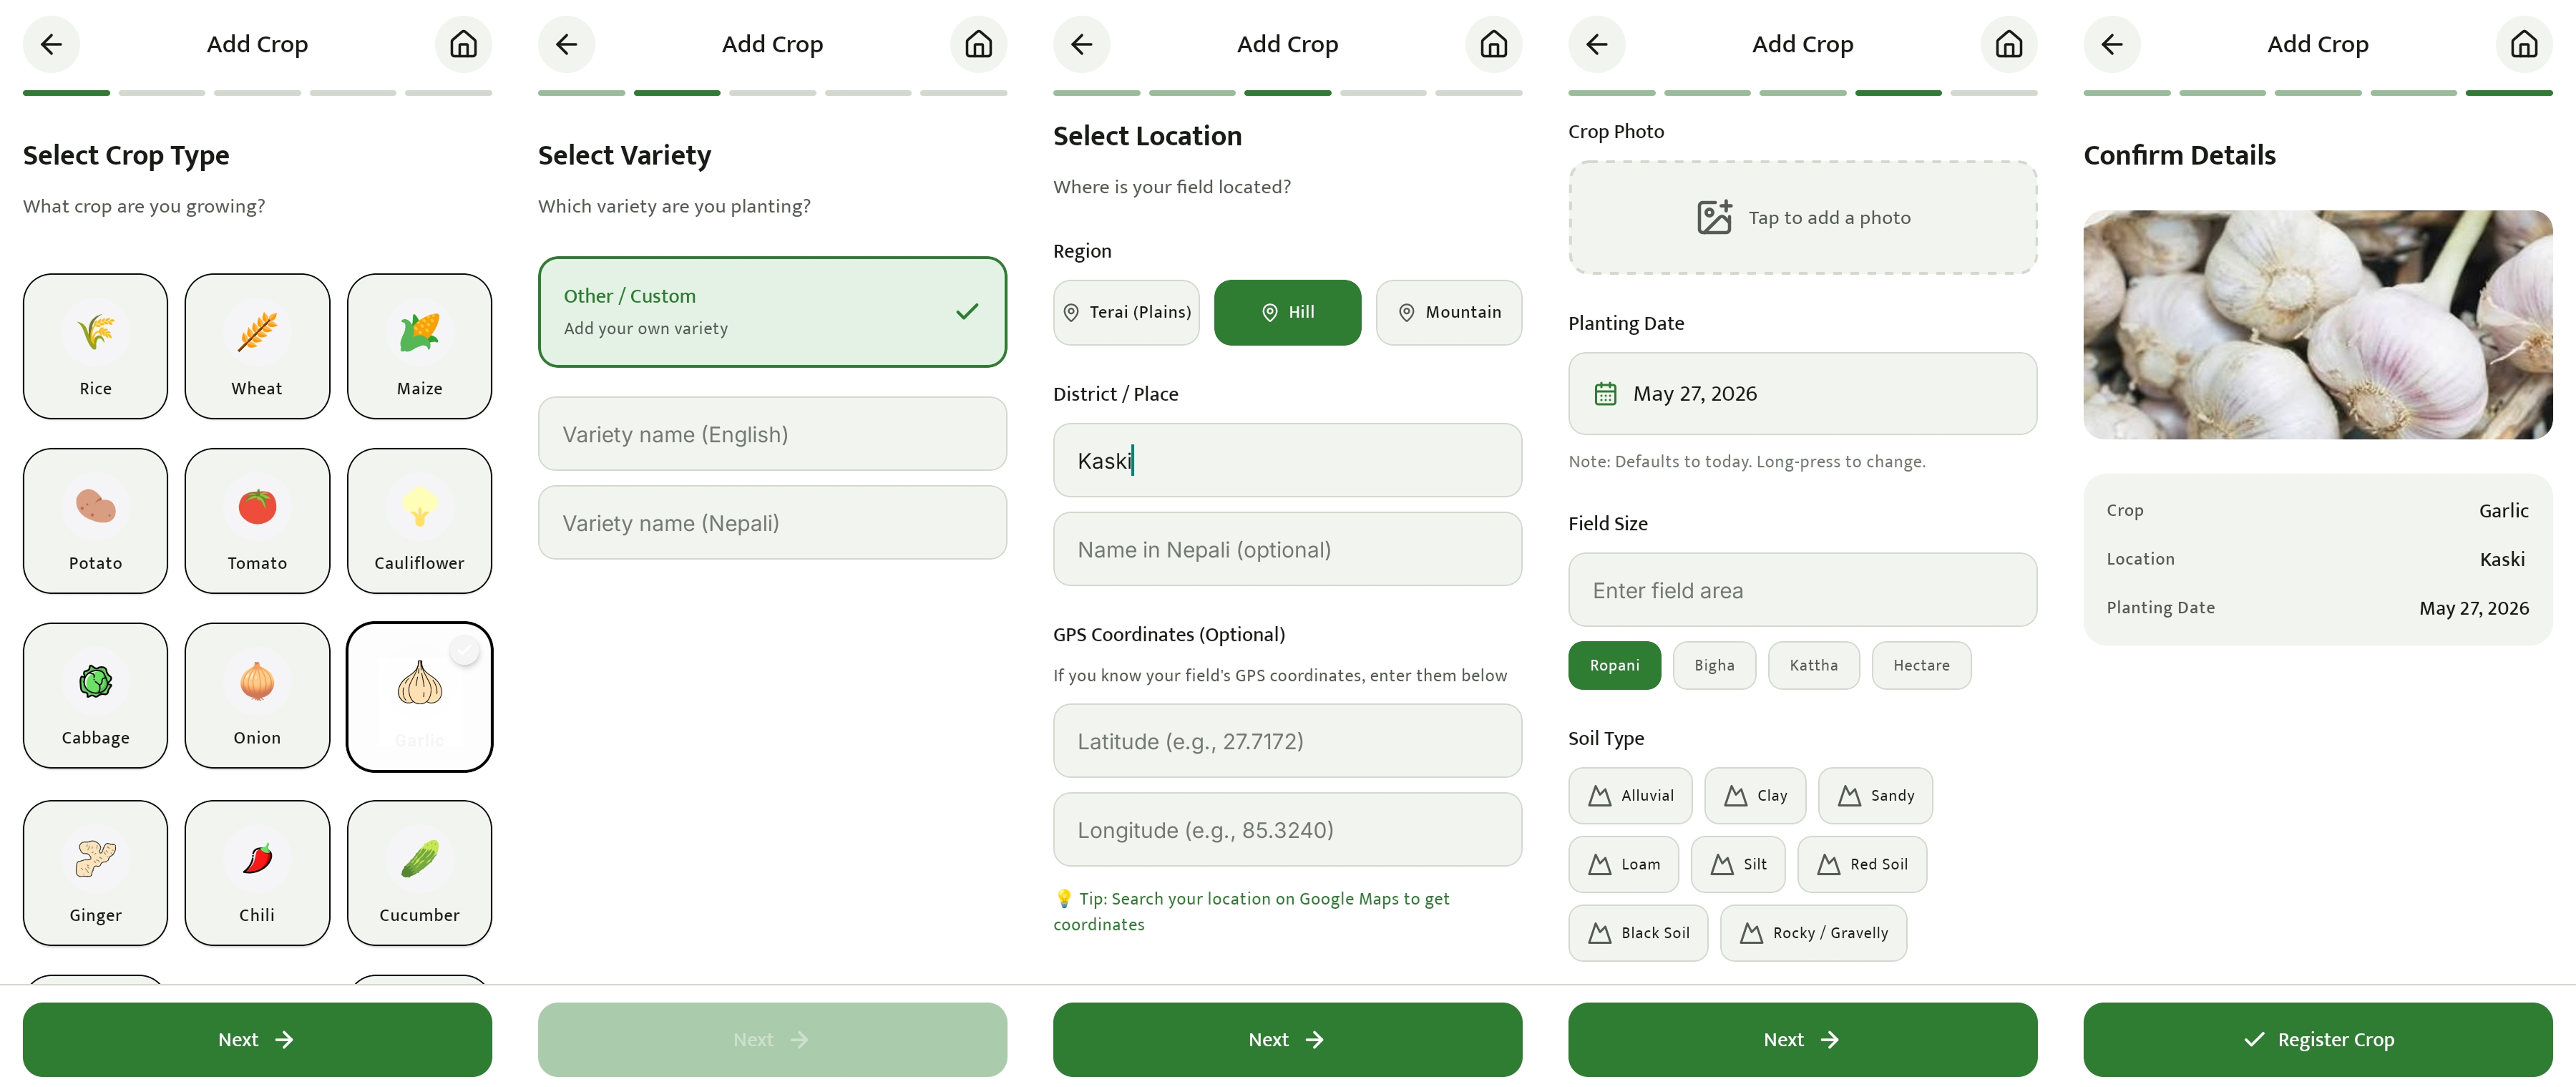
\includegraphics[height=0.4\textheight,keepaspectratio,width=\linewidth]{data/krishi_vaidya_mobile_app_data/add_crops/add_crop.png}
\caption{Crop registration screenshot.}
\label{fig:mobile-crop-registration}
\end{figure}

\subsubsection{Model Deployment and Verification}

The app packages TFLite model assets in int8, fp16, and fp32 precision variants, exposing model
precision as a user-facing setting. The TFLite service attempts GPU loading with CPU fallback,
and supports runtime precision switching. The mobile application correctly enforces the 11-class
plant-part taxonomy from the YOLO training pipeline, confirming alignment between exported models
and the inference parser.

Source inspection and physical-device testing verify architecture, navigation, persistence,
diagnosis flow, offline recovery, and model-asset loading. Broader device-fragmentation
testing and expanded automated app-level tests remain future work.

\ChapterSubsection{Integrated System Discussion}

\subsubsection{End-to-End Integration Outcome}

The integrated system combines mobile capture, backend orchestration, VLM prediction, structured
advisory generation, and local result handling through the architecture described in Chapter~4.
The key integration outcome is clean separation of responsibilities: the mobile app never calls
the VLM or advisory services directly, the backend never surfaces raw model text, and each
boundary validates or normalizes data before passing it forward.

End-to-end validation used a distributed deployment---VLM on Lightning.ai, database on Supabase,
backend via ngrok---that verified the complete request lifecycle including offline queue
recovery. The offline path writes scans to the local queue, creates pending history records, and
can return cached advisories while retaining queued scans for later cloud processing.

\subsubsection{Limitations and Evidence Gaps}

The VLM was intentionally constrained by training cost, and the backend schema masks raw outputs
but cannot by itself convert a three-epoch model into a mature diagnostic authority. Automated
integration test coverage extends to the scan domain and VLM API behavior; secondary workflow
tests and concurrent-load scaling remain future work. Complete bidirectional offline
synchronization is implemented as infrastructure but awaits full backend handler coverage.

\ChapterSubsection{Cross-System Results Discussion and Limitations}

\subsubsection{Synthesis of Major Results}

Table~\ref{tab:cross-system-result-synthesis} summarizes the strongest result and main caution
for each system area. The YOLO subsystem provides the strongest quantitative evidence, including
threshold analysis and deployment profiling. The VLM subsystem delivers a complete fine-tuning
pipeline while exposing parseability as a critical bottleneck. The backend implements an
orchestration boundary with schema-enforced advisories. The mobile app implements a local-first
\parencite{kleppmannLocalFirst2019} farmer-facing interface with offline-aware queuing and
localized result rendering.

The strongest overarching contribution is architectural. By constructing a pipeline from field
image capture to schema-validated bilingual advisory, Krishi Vaidya makes visible the ``hidden
technical debt'' \parencite{sculleyMLTechDebt2015} between a trained classifier and a deployed
application---the defensive validation, structured assembly, resilient persistence, and
linguistic translation that much of the existing literature omits
\parencite{liu2021plantDiseaseReview, wangAgriLLaVA2024}.

{\small \renewcommand{\arraystretch}{1.3}
\begin{xltabular}{\textwidth}{@{} l L L @{}}
\caption{Cross-system result synthesis}\label{tab:cross-system-result-synthesis}\\
\toprule
\textbf{System area} & \textbf{Strongest result} & \textbf{Main caution} \\
\midrule
\endfirsthead
\multicolumn{3}{l}{\textit{(continued from previous page)}} \\
\toprule
\textbf{System area} & \textbf{Strongest result} & \textbf{Main caution} \\
\midrule
\endhead
\midrule
\multicolumn{3}{r}{\textit{(continues on next page)}} \\
\endfoot
\bottomrule
\endlastfoot
YOLO detector & Quantitative detection and deployment evidence supports manuscript claims & Wider device profiling and long-term monitoring remain production extensions \\
VLM model & Dataset, fine-tuning, and validation pipeline complete and documented & Prediction accuracy and parseability weak on the independent test set \\
Backend API & Structured diagnosis orchestration, validation, and scan tests exist & Broader route and diagnosis-integration tests can be expanded \\
Mobile app & Complete farmer workflow verified on physical Android devices & Device-fragmentation testing remains future work \\
Integration & End-to-end diagnosis verified across mobile, backend, VLM, and advisory layers & Automated coverage can be broadened across secondary workflows \\
\end{xltabular}
}

\subsubsection{Model-Level Interpretation}

The YOLO model is the most mature ML component, backed by training dynamics, threshold analysis,
deployment comparison, and per-class error analysis. The VLM work is substantial in
scope---dataset construction, LoRA fine-tuning, quantized training, inference infrastructure,
and structured evaluation---but its independent prediction metrics show that the three-epoch
model should not serve as a final diagnostic authority. The low evaluation loss and high token
accuracy confirm a technically promising adaptation direction; the limitation is the present
training and decoding constraint, not the absence of a viable VLM pathway.

\subsubsection{System-Level Interpretation}

The backend and mobile results confirm that Krishi Vaidya was engineered as a system rather than
an isolated experiment. The agreement between implemented architecture and distributed runtime
validation confirms platform viability. Reliability controls---image validation, readiness
checks, JWT authentication, schema enforcement, offline queuing---limit how far an invalid or
unavailable component can propagate through the user-facing workflow, though they do not resolve
agronomic safety challenges such as model uncertainty, field-image variability, and pesticide
recommendation risk.

\subsubsection{Current Limitations}

Table~\ref{tab:cross-system-limitations} organizes limitations and improvement actions across
five groups. The project can claim a modular system with YOLO, VLM, backend, mobile, and
integration components, documented with quantitative analysis. It cannot yet claim high VLM
accuracy, agronomic field testing, or production-scale deployment. Maintaining this boundary
strengthens the thesis by clearly separating implementation evidence from deployment readiness.

{\small \renewcommand{\arraystretch}{1.3}
\begin{xltabular}{\textwidth}{@{} l L L @{}}
\caption{Cross-system limitations and improvement actions}\label{tab:cross-system-limitations}\\
\toprule
\textbf{Limitation group} & \textbf{Current limitation} & \textbf{Improvement action} \\
\midrule
\endfirsthead
\multicolumn{3}{l}{\textit{(continued from previous page)}} \\
\toprule
\textbf{Limitation group} & \textbf{Current limitation} & \textbf{Improvement action} \\
\midrule
\endhead
\midrule
\multicolumn{3}{r}{\textit{(continues on next page)}} \\
\endfoot
\bottomrule
\endlastfoot
VLM reliability & Three-epoch training shows promising adaptation but limited prediction and parseability & Extend training, add constrained decoding, improve dataset balance, strengthen evaluation \\
Backend test coverage & Automated testing covers the scan domain; secondary routes manually verified & Expand tests for remaining route domains and external diagnosis branches \\
Mobile validation & Physical-device workflows verified; extreme fragmentation untested & Conduct device-compatibility studies across budget Android phones \\
Offline synchronization & Core queue recovery verified; full table sync remains limited & Add backend handlers for remaining secondary tables \\
Agronomic safety & Generated advice can still be uncertain or unsafe without review & Preserve confidence tiers, safety warnings, source links, and expert consultation guidance \\
\end{xltabular}
}
